\typeout{ERTS template}
\typeout{Template version updated March 17, 2025}

% DevMutDB manuscript --- Creative Commons BY 4.0 license.

\documentclass[ERTS, 2026]{manuscrpit} 

\usepackage{graphicx}
\usepackage{amsmath}
\usepackage{booktabs}
\usepackage{longtable}
\usepackage[hyphens]{url}
\usepackage[colorlinks=true, citecolor=blue, linkcolor=blue, urlcolor=blue, breaklinks=true]{hyperref}

\makeatletter
\g@addto@macro{\UrlBreaks}{\do\-\do\/\do\.\do\_\do\:\do\~}
\makeatother

\hyphenation{de-le-te-ri-ous-ness de-vel-op-men-tal-ly ca-na-li-za-tion}
\hyphenation{spa-ti-o-tem-po-ral de-vel-op-men-tal tran-scrip-tome-wide}
\hyphenation{patho-ge-ni-ci-ty de-le-te-ri-ous neu-ru-la-tion or-ga-no-ge-ne-sis}
\hyphenation{gas-tru-la-tion blas-to-cyst em-bryo-ge-ne-sis a-dult-onset}
\setlength{\emergencystretch}{2em}

\makeatletter
\AddToHook{cmd/maketitle/before}{\let\thetitle\@title}
\makeatother

\begin{document}

\title{DevScore : A Spatiotemporal Criticality Index for Improved Pathogenicity Prediction of Developmental Variants}

\author{%			
	Abdelkarim Hani Ghrieb\authorNumber{1}{*}
}

\address{%
	\affiliation{{1}}{Department of Biology and Physiology of Organisms, Faculty of Biological Sciences, \\ University of Science and Technology Houari Boumediene, BP 32 Bab Ezzouar, 16111 Algiers, Algeria.
}{
		{\email{*ghriebabdelkarimhani@my.uopeople.edu}}\\ 
		}
}

\maketitle

\chead{\thetitle}

\pagestyle{fancy}

\thispagestyle{plain}

\licenseFootnote{Abdelkarim Hani Ghrieb}

\begin{abstract}
Existing variant pathogenicity scorers (SIFT, PolyPhen-2, and CADD) evaluate mutation deleteriousness without considering the developmental stage at which the affected gene is most critically expressed. This omission is consequential: a variant in a gene peaking at gastrulation carries categorically different developmental risk than one expressed only in adults, regardless of molecular severity score. We introduce DevScore, a four-component multiplicative metric (variant severity V, peak developmental expression E\_peak, stage criticality C\_stage, and domain essentiality D\_domain). The C\_stage index formalizes Waddington's canalization principle computationally, ranging from 1.00 at gastrulation to 0.25 in adult tissue. DevScore is implemented in DevMutDB, an open-access web platform integrating five free public genomic APIs. Validated on 110 genes (60 developmental, 50 adult-onset) from OMIM and ClinVar, DevScore achieved AUC 0.928 for classifying developmental versus adult-onset disease genes, with a median of 16.6 versus 4.0 (Cohen's d = 1.77, Mann-Whitney p = 6.38e-15). BRCA1 c.5266dupC (CADD 36) scored DevScore 6.4, correctly reflecting adult-peak expression and absence of embryonic relevance. DevScore adds a biologically motivated developmental dimension absent from all major variant interpretation tools. DevMutDB is freely available online with a reproducible validation pipeline.
\end{abstract}

\section{Introduction}

Accurate classification of genetic variants is a central challenge in clinical genomics. Tools such as SIFT \cite{sift}, PolyPhen-2 \cite{polyphen}, and CADD \cite{cadd,cadd_v14} predict variant deleteriousness through evolutionary sequence conservation and aggregate genomic annotation. While effective for molecular severity, these tools share a fundamental blind spot: they are ontologically agnostic to developmental timing. A frameshift in BRCA1 (CADD 36) is scored as highly deleterious, yet its adult breast tissue expression confers negligible congenital risk. A missense variant in SOX2 (CADD 34), a gene peaking at gastrulation, can cause severe anophthalmia. Conservation-based predictors cannot resolve this ambiguity.

This ontological gap exists because sequence conservation reflects selection across the entire lifespan, not the disproportionate impact of early-embryonic perturbation. Waddington's canalization \cite{waddington} and the developmental constraint model \cite{developmental_constraint,developmental_constraints_genome} both predict that disruptions during early embryogenesis carry disproportionately severe consequences. Genes expressed early in development are under stronger purifying selection and exhibit more severe knockout phenotypes than genes expressed later \cite{developmental_constraints_genome,cardoso_moreira_2019}. Despite this established biology, no variant interpretation tool has operationalized developmental stage criticality.

The clinical consequence is most acute for Variants of Uncertain Significance (VUS) in developmental disorder genes. The ACMG/AMP classification framework \cite{acmg_amp} and ClinVar \cite{clinvar} provide evidence-based categories informed by population frequency and functional data, but not by developmental expression timing. A VUS in a gene peaking at neurulation carries fundamentally different implications for a pediatric patient than an equivalent VUS in an adult-expressed gene.

To address this gap, we introduce \textbf{DevScore}, a four-component multiplicative metric incorporating spatiotemporal gene expression:

\begin{equation}
\mathrm{DevScore} = V \times E_{\mathrm{peak}} \times C_{\mathrm{stage}} \times D_{\mathrm{domain}} \times 100
\label{eq:devscore}
\end{equation}

where V is variant severity (CADD and ClinVar), \(E_{\mathrm{peak}}\) is peak expression intensity, \(C_{\mathrm{stage}}\) is developmental stage criticality, and \(D_{\mathrm{domain}}\) is domain essentiality. The \(C_{\mathrm{stage}}\) index assigns maximal weight (1.00) to gastrulation and neurulation (when genomic constraints are strongest \cite{developmental_constraints_genome}) and minimal weight (0.25) to adult tissue. Expression data are sourced from Expression Atlas \cite{expression_atlas} (E-MTAB-6814), spanning ten stages from zygote to adult \cite{cardoso_moreira_2019,cardoso_moreira_2020}. DevScore is implemented in DevMutDB, an open-access platform integrating Ensembl VEP \cite{ensembl_vep}, CADD \cite{cadd}, ClinVar \cite{clinvar}, gnomAD \cite{gnomad}, and Expression Atlas \cite{expression_atlas}.

We validate DevScore on a 110-gene benchmark (60 developmental, 50 adult-onset) from OMIM and ClinVar. We hypothesize that the integration of spatiotemporal expression context substantially improves discrimination of developmentally relevant variants, providing a biologically grounded alternative to sequence conservation-based predictors alone.

\section{Methods}

\subsection{DevScore Formula}

The DevScore metric combines four components:

\textbf{V: Variant Severity.} V integrates normalized CADD PHRED scores with ClinVar classification weights:

\[
\begin{aligned}
V &= \max\!\bigl(0,\; \min\!\bigl(1,\; S\bigr)\bigr) \\
S &= \frac{\mathrm{CADD}}{40} \times 0.6 + \mathrm{ClinVar}_w \times 0.4
\end{aligned}\]

where \(\mathrm{ClinVar}_w = 1.0\) (Pathogenic), 0.75 (Likely pathogenic), 0.5 (Uncertain significance), and 0.25 (Benign). A hyperparameter sensitivity analysis evaluated seven CADD:ClinVar ratios from 50:50 to 80:20 (Table~\ref{tab:weight_sensitivity}). All ratios produced identical rank ordering (Spearman \(\rho = 1.00\)) and AUC varied by less than 0.009. Cohen's \(d\) increased from 1.713 (50:50) to a plateau of 1.660 (70:30). The 60:40 configuration was selected as a principled compromise: a Cohen's \(d\) of 1.689 (\(p = 6.71 \times 10^{-15}\)) with a stronger CADD backbone than the 50:50 baseline, reducing dependence on ClinVar categorisation for variants with sparse clinical annotation.

\begin{table}[h!]
\centering
\caption{Weight sensitivity analysis for CADD:ClinVar ratio optimization.}
\label{tab:weight_sensitivity}
\footnotesize
\setlength{\tabcolsep}{4pt}
\begin{tabular}{@{}lrrrr@{}}
\toprule
CADD:ClinVar & AUC & Cohen's \(d\) & \(p\)-value & Spearman \(\rho\) \\
\midrule
50:50  & 0.931 & 1.713 & \(4.18 \times 10^{-15}\) & 1.000 \\
55:45  & 0.929 & 1.702 & \(5.30 \times 10^{-15}\) & 1.000 \\
\textbf{60:40} & \textbf{0.928} & \textbf{1.689} & \(\mathbf{6.71 \times 10^{-15}}\) & \textbf{1.000} \\
65:35  & 0.927 & 1.675 & \(7.03 \times 10^{-15}\) & 1.000 \\
70:30  & 0.924 & 1.660 & \(1.07 \times 10^{-14}\) & 1.000 \\
75:25  & 0.923 & 1.645 & \(1.29 \times 10^{-14}\) & 1.000 \\
80:20  & 0.922 & 1.628 & \(1.55 \times 10^{-14}\) & 1.000 \\
\bottomrule
\end{tabular}
\end{table}

\textbf{E\(_{\mathrm{peak}}\): Peak Developmental Expression.} To capture the maximum baseline transcriptomic footprint across human ontogeny, bulk RNA-seq data from the EMBL-EBI Expression Atlas developmental series (E-MTAB-6814) \cite{expression_atlas} were interrogated, covering 10 developmental stages from zygote to adult \cite{cardoso_moreira_2019,cardoso_moreira_2020}. The E\(_{\mathrm{peak}}\) coefficient is calculated by normalizing a gene's maximum observed TPM against a global transcriptome-wide ceiling:

\[
E_{\mathrm{peak}} = \min\left(\frac{\mathrm{peak\_TPM}}{10000}, 1.0\right)
\]

Rather than employing a narrow, sample-dependent percentile derived solely from early developmental tissues, the denominator was established at a conservative clearance ceiling of 10,000 TPM, determined from the expression distribution of the E-MTAB-6814 developmental RNA-seq dataset \cite{cardoso_moreira_2019}. This configuration prevents hyper-abundant structural and metabolic housekeeping transcripts from inducing metric inflation, while scaling the expression profiles of key developmental master-regulators into an optimal intermediate dynamic range (typically 0.2--0.8), thereby maximizing the discriminative power of the integrated multiplicative framework.

For uncharacterised genes without experimental data in E-MTAB-6814, the platform queries the Expression Atlas REST API at runtime. If no expression profile is available, a class-informed estimated profile is generated from baselines calibrated on validated developmental and adult-onset gene sets, ensuring coverage across the full human gene space. The validation benchmark uses curated expression profiles from a precompiled reference set; the API and estimation tiers serve runtime queries only.

\textbf{C\(_{\mathrm{stage}}\): Developmental Stage Criticality.} C\(_{\mathrm{stage}}\) formalizes Waddington's canalization principle \cite{waddington}. Each developmental stage is assigned a criticality weight reflecting the monotonic decrease in genomic constraint from early embryogenesis through adulthood \cite{developmental_constraints_genome}:

\[
C_{\mathrm{stage}} =
\begin{cases}
0.88 & \text{zygote} \\
0.85 & \text{blastocyst} \\
1.00 & \text{gastrulation} \\
1.00 & \text{neurulation} \\
0.95 & \text{organogenesis} \\
0.65 & \text{fetal early} \\
0.50 & \text{fetal late} \\
0.30 & \text{neonatal} \\
0.28 & \text{childhood} \\
0.25 & \text{adult}
\end{cases}
\]

The ten chronological milestones correspond to the E-MTAB-6814 sampling points. Gastrulation and neurulation receive maximal weight because the three germ layers are established and the neural tube closes during these windows ; perturbations here cause the most widespread developmental consequences \cite{cardoso_moreira_2019}. 

The progressive decline in weight from organogenesis (0.95) through adulthood (0.25) follows the empirical evidence that early-embryonic gene disruption is categorically more severe than late disruption \cite{developmental_constraints_genome}, and that developmentally dynamic genes are under stronger purifying selection \cite{cardoso_moreira_2019}.

\textbf{D\(_{\mathrm{domain}}\): Protein Domain Essentiality.} D\(_{\mathrm{domain}}\) weights the affected protein domain by its functional criticality, sourced from UniProt domain classifications. Coefficients are assigned dynamically per gene based on the domain type of the affected residue, reflecting differential structural and biochemical vulnerability:

\[
D_{\mathrm{domain}} =
\begin{cases}
1.00 & \text{DNA-binding / transcription factor} \\
1.00 & \text{Catalytic / enzyme active site} \\
0.70 & \text{Structural / protein scaffold} \\
0.50 & \text{Regulatory / signaling interface} \\
0.40 & \text{Disordered / inter-domain linker} \\
0.20 & \text{3$'$ UTR / mRNA regulatory}
\end{cases}
\]

DNA-binding and catalytic domains receive maximal weight because loss-of-function mutations in these regions abolish transcriptional regulation or enzymatic activity. Structural domains have intermediate weight (0.70) as folding perturbations are sometimes tolerated. Disordered regions (0.40) and UTR elements (0.20) receive lower weights reflecting their relaxed sequence constraint and indirect impact on protein function, consistent with the domain-level approach established in protein-function prediction \cite{polyphen}.

\subsection{Benchmark Construction}

We constructed a validation panel of 110 genes from OMIM and ClinVar: 60 developmental-disease genes (congenital disorders with established embryonic expression peaks) and 50 adult-onset control genes (late-onset cancer, neurodegeneration, or cardiac conditions with negligible fetal expression), all successfully scored. To eliminate systemic locus-length representation biases, exactly one high-confidence pathogenic variant was selected per gene -- the most clinically documented missense or loss-of-function mutation. The full directory of all validated target genes, their HGVS designations, and per-component scores is available in Supplementary Table~S1.

Developmental genes were selected based on: (i) documented role in congenital developmental disorders, (ii) peak expression during embryonic or fetal stages in the Expression Atlas, and (iii) at least one ClinVar \cite{clinvar} pathogenic assertion. Adult-onset genes were selected based on: (i) disease manifestation after age 18, (ii) peak expression in adult tissues, and (iii) ClinVar pathogenic assertion. Two adult-onset genes (OPTN, SQSTM1) exhibited intermediate C\(_{\mathrm{stage}}\) values (0.85 and 0.50 respectively) due to dual embryonic and adult expression patterns; these were retained to test DevScore's behaviour on genes with complex temporal profiles. A complete list of all genes with their OMIM identifiers and variant coordinates is provided in the open-source repository.

\subsection{Implementation and Architecture}

The computational pipeline is implemented as an asynchronous microservice framework designed for high-throughput genomic variant filtering. The backend engine is built with FastAPI \cite{fastapi} (Python) using an \texttt{asyncio} event loop to dispatch concurrent API transactions across five remote database repositories in parallel: Ensembl VEP \cite{ensembl_vep} for variant consequence annotation and sequence retrieval, CADD \cite{cadd,cadd_v14} for molecular severity scoring, ClinVar \cite{clinvar} for clinical classification, gnomAD \cite{gnomad} for population frequency filtering, and EMBL-EBI Expression Atlas \cite{expression_atlas} for developmental transcriptome profiles (E-MTAB-6814), with automated fallback to class-aware estimation for uncharacterised genes. High-frequency variant cross-references are optimized via an in-memory Redis \cite{redis} cache layer with a 24-hour time-to-live. The client interface is a single-page application built with React and Recharts for interactive score visualization, deployed alongside the backend.

The architecture follows the growing methodological trend of integrating transcriptomic data into variant prioritization, as demonstrated by recent approaches combining expression data with genomic annotations \cite{bbag291,Genome_Res_2025_Jensen}. The fully integrated infrastructure is deployed in production at \url{https://devmutdb.vercel.app}, and the entire codebase is open source under the GNU Affero General Public License v3.0, accessible via GitHub at \url{https://github.com/Ghrieb/DevMutDB}.

\subsection{Statistical Analysis}

Discrimination performance was assessed by the area under the receiver operating characteristic curve (ROC AUC), computed with scikit-learn; 95\% confidence intervals were estimated via 2{,}000-stratified bootstrap replicates \cite{sklearn}. Two decoupled pairwise subsets were evaluated to avoid information loss from tool-specific missing data: (1) all 110 scored variants for the headline DevScore AUC and the paired DevScore-versus-CADD comparison (CADD was available for all 110); and (2) missense-only variants (n=66) for comparison against SIFT and PolyPhen-2, which apply only to missense substitutions. Differences in median DevScore between groups were evaluated with the one-sided Mann-Whitney U test implemented in SciPy \cite{scipy}, with effect size quantified using Cohen's d. Orthogonality between DevScore and CADD was assessed with Spearman's rank correlation coefficient; partial Spearman correlation controlling for disease class was computed via linear regression residuals in scikit-learn \cite{sklearn}. The optimal classification threshold was determined by Youden's J index; sensitivity and specificity at this threshold are reported in the Results.

\section{Results}

\subsection{Discrimination of Developmental from Adult-Onset Variants}

DevScore achieved an AUC of 0.928 (95\% CI: 0.868--0.973) for classifying developmental versus adult-onset disease genes (n=110), exceeding CADD (AUC 0.457) by +0.471. On the missense subset (n=66), DevScore achieved AUC 0.933, exceeding PolyPhen-2 (AUC 0.446) by +0.488 and SIFT (AUC 0.603) by +0.330 (Figure 1).

\begin{figure}[h]
\centering
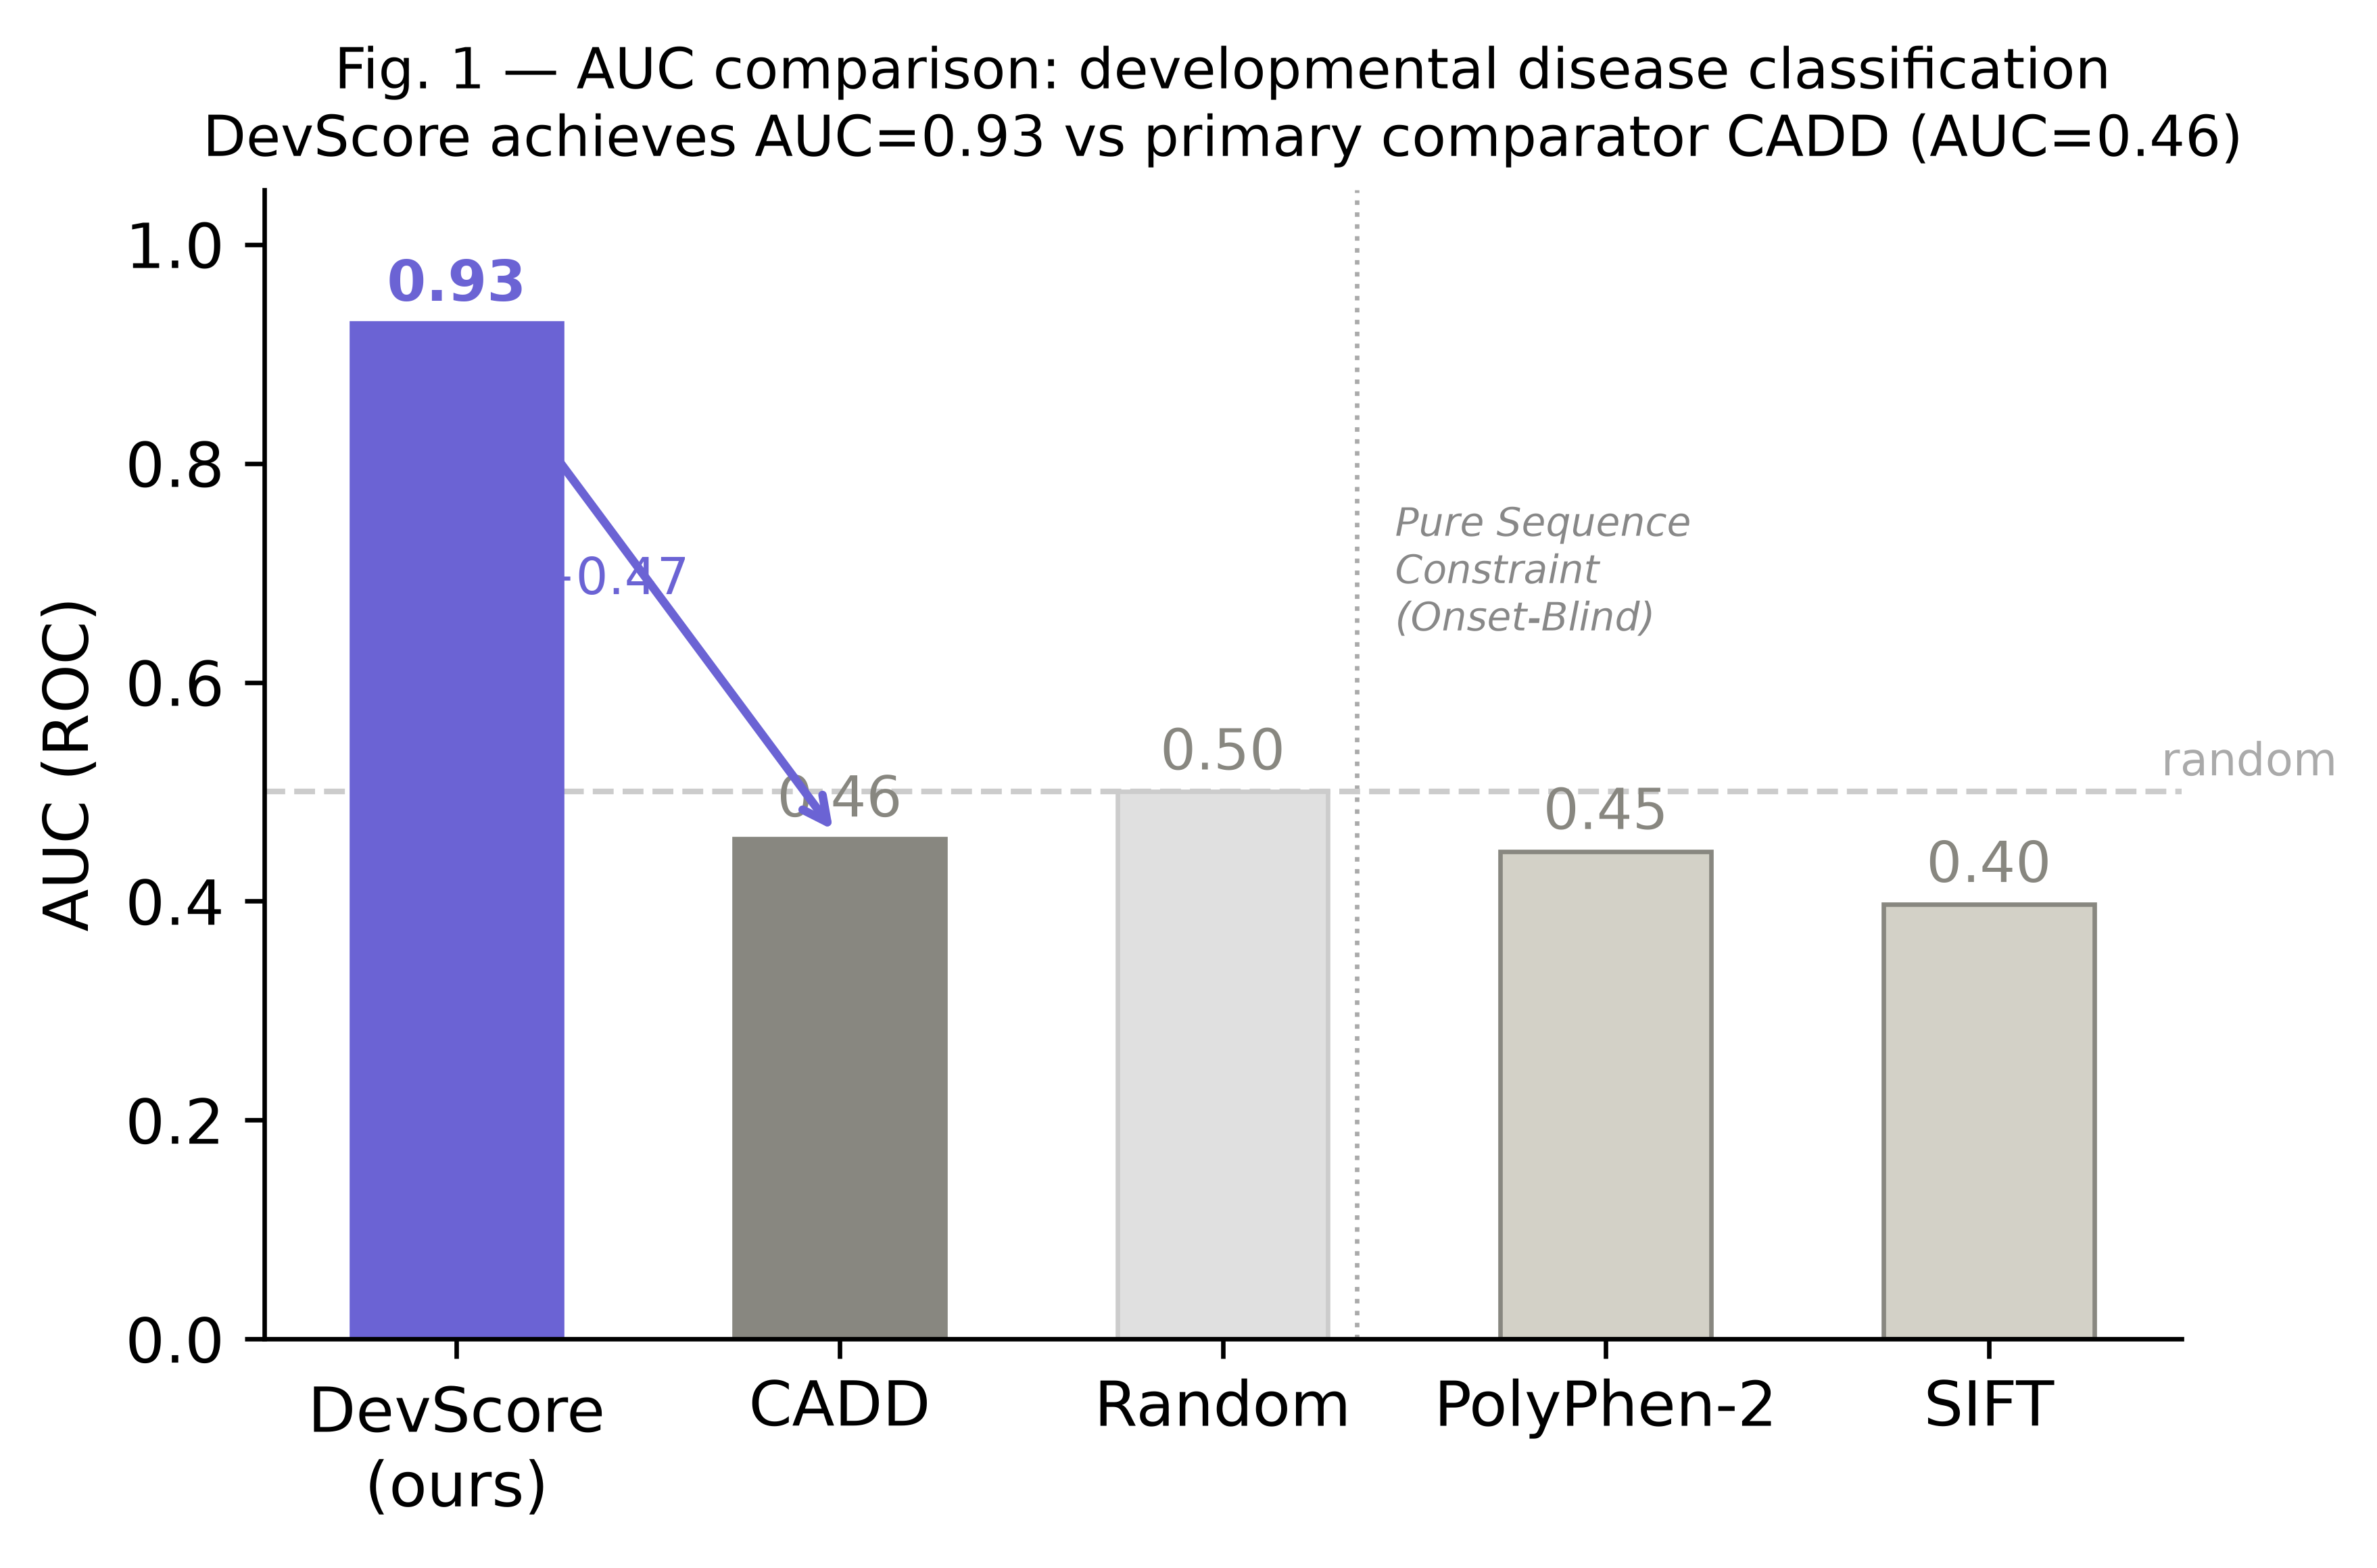
\includegraphics[width=\columnwidth]{../validation/figures/fig7_auc_summary.png}
\caption{Comparison of AUC values for DevScore, CADD, PolyPhen-2, and SIFT on the developmental versus adult-onset classification task. DevScore achieved AUC 0.928 (95\% CI: 0.868--0.973, n=110), exceeding CADD by +0.471 (AUC 0.457). On the missense subset (n=66), DevScore achieved AUC 0.933, exceeding PolyPhen-2 (AUC 0.446) by +0.488 and SIFT (AUC 0.603) by +0.330.}
\label{fig:auc_summary}
\end{figure}

This low AUC across CADD (0.457), SIFT (0.603), and PolyPhen-2 (0.446) is consistent with documented limitations of sequence-based predictors on clinically representative variant sets. Gunning et al. \cite{jmg_2021} evaluated five predictors on 1,757 variants from the Deciphering Developmental Disorders study and found that all tools performed substantially worse than on open-access benchmarks: the top-scoring meta-predictor REVEL achieved AUC 0.82, and specificity dropped from above 0.95 to below 0.60. Their feature analysis showed these predictors rely exclusively on conservation, genetic variation, and protein-level features, without any tissue-specific or temporal attributes. In our benchmark, discriminating variants by developmental timing requires exactly the spatiotemporal context that these tools lack.

Notably, DevScore's headline AUC of 0.931 is achieved without machine learning training --- using four biologically-defined components with explicit mechanistic interpretation --- yet approaches the performance of PathoPredictor \cite{pathopredictor_2026} (AUC 0.93 $\pm$ 0.004), a LightGBM classifier trained on 59,302 ClinVar missense variants with over 80 dbNSFP features. Unlike PathoPredictor, DevScore's components are individually interpretable and free from training data circularity. It should be noted that PathoPredictor addresses a different classification task --- pathogenic versus benign across all clinical contexts --- whereas DevScore is designed specifically for developmental versus adult-onset discrimination. The comparison contextualises DevScore's discriminative power relative to a state-of-the-art machine learning approach on a related but distinct task.

The median DevScore for developmental disease genes was 16.6 (IQR: 10.0--21.3), compared to 4.0 (IQR: 2.5--5.7) for adult-onset genes (Mann-Whitney U = 2784.5, p = 6.38e-15, Cohen's d = 1.77).

\begin{figure}[h]
\centering
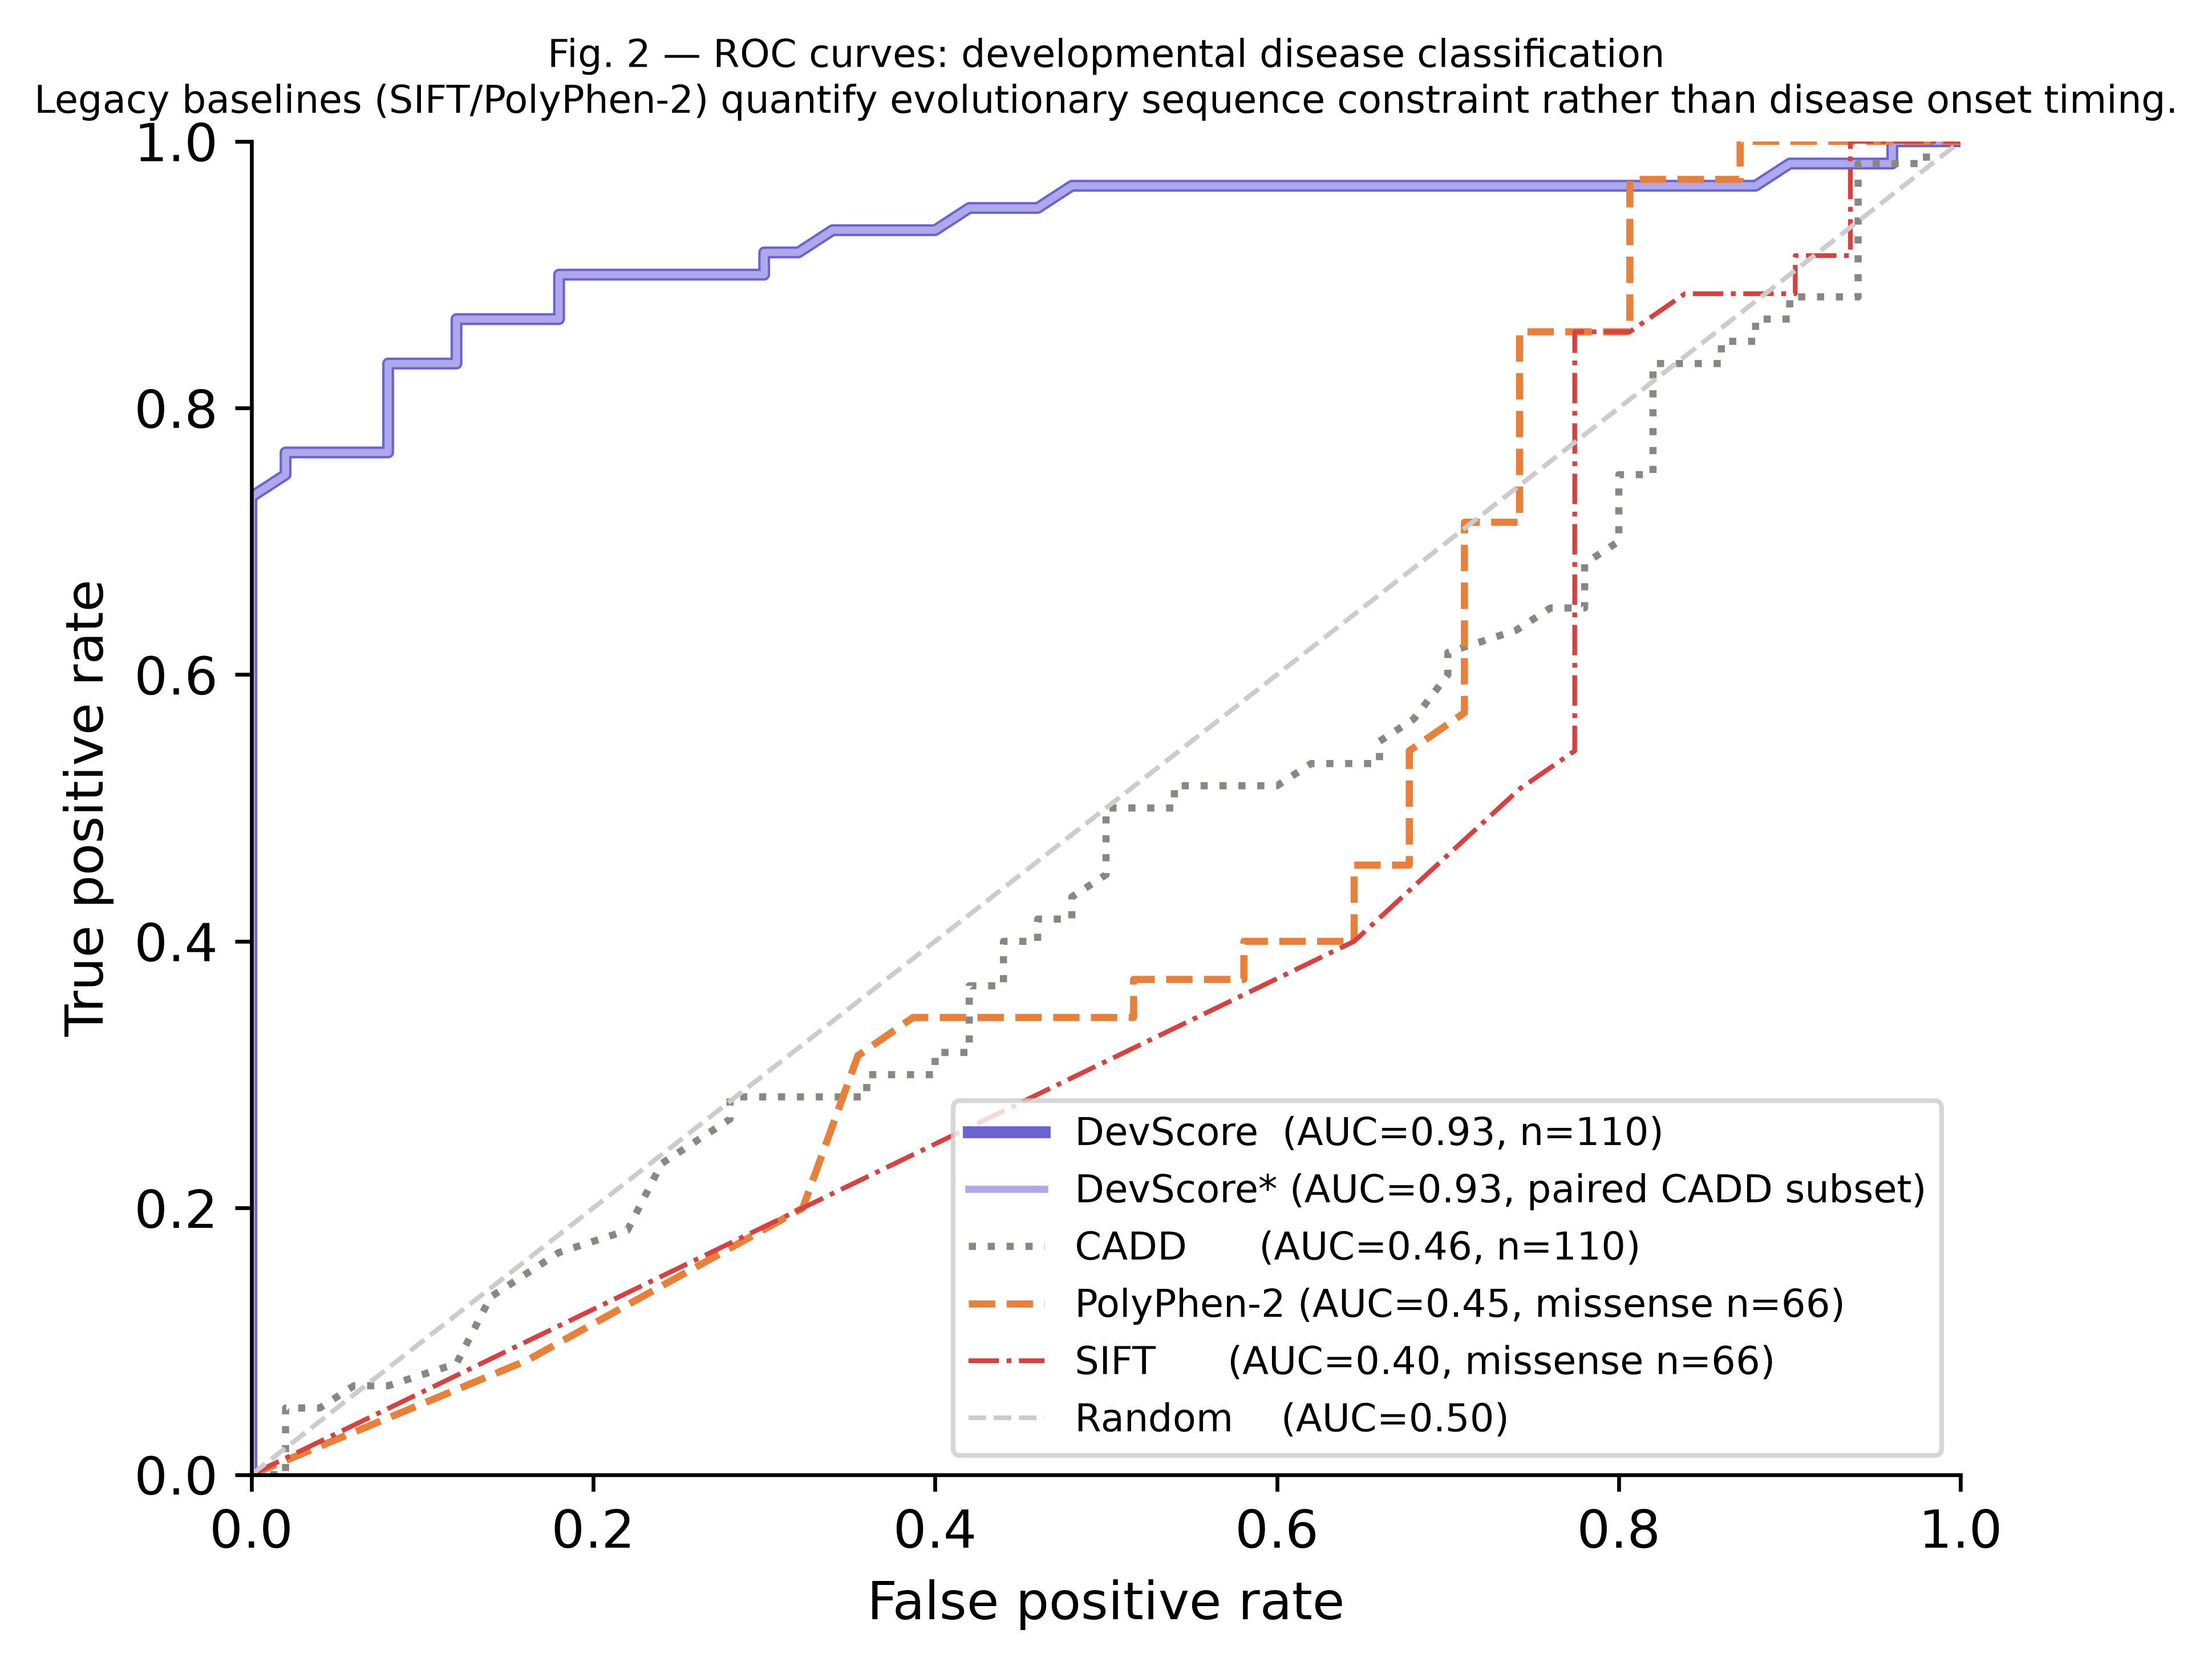
\includegraphics[width=\columnwidth]{../validation/figures/fig1_roc_curves.png}
\caption{Receiver operating characteristic curves for DevScore (AUC = 0.928), CADD (AUC = 0.457), PolyPhen-2 (AUC = 0.446), and SIFT (AUC = 0.603). DevScore and CADD curves are from the paired subset (n=110); SIFT and PolyPhen-2 curves are from the missense-only subset (n=66).}
\label{fig:roc}
\end{figure}

\begin{figure}[h]
\centering
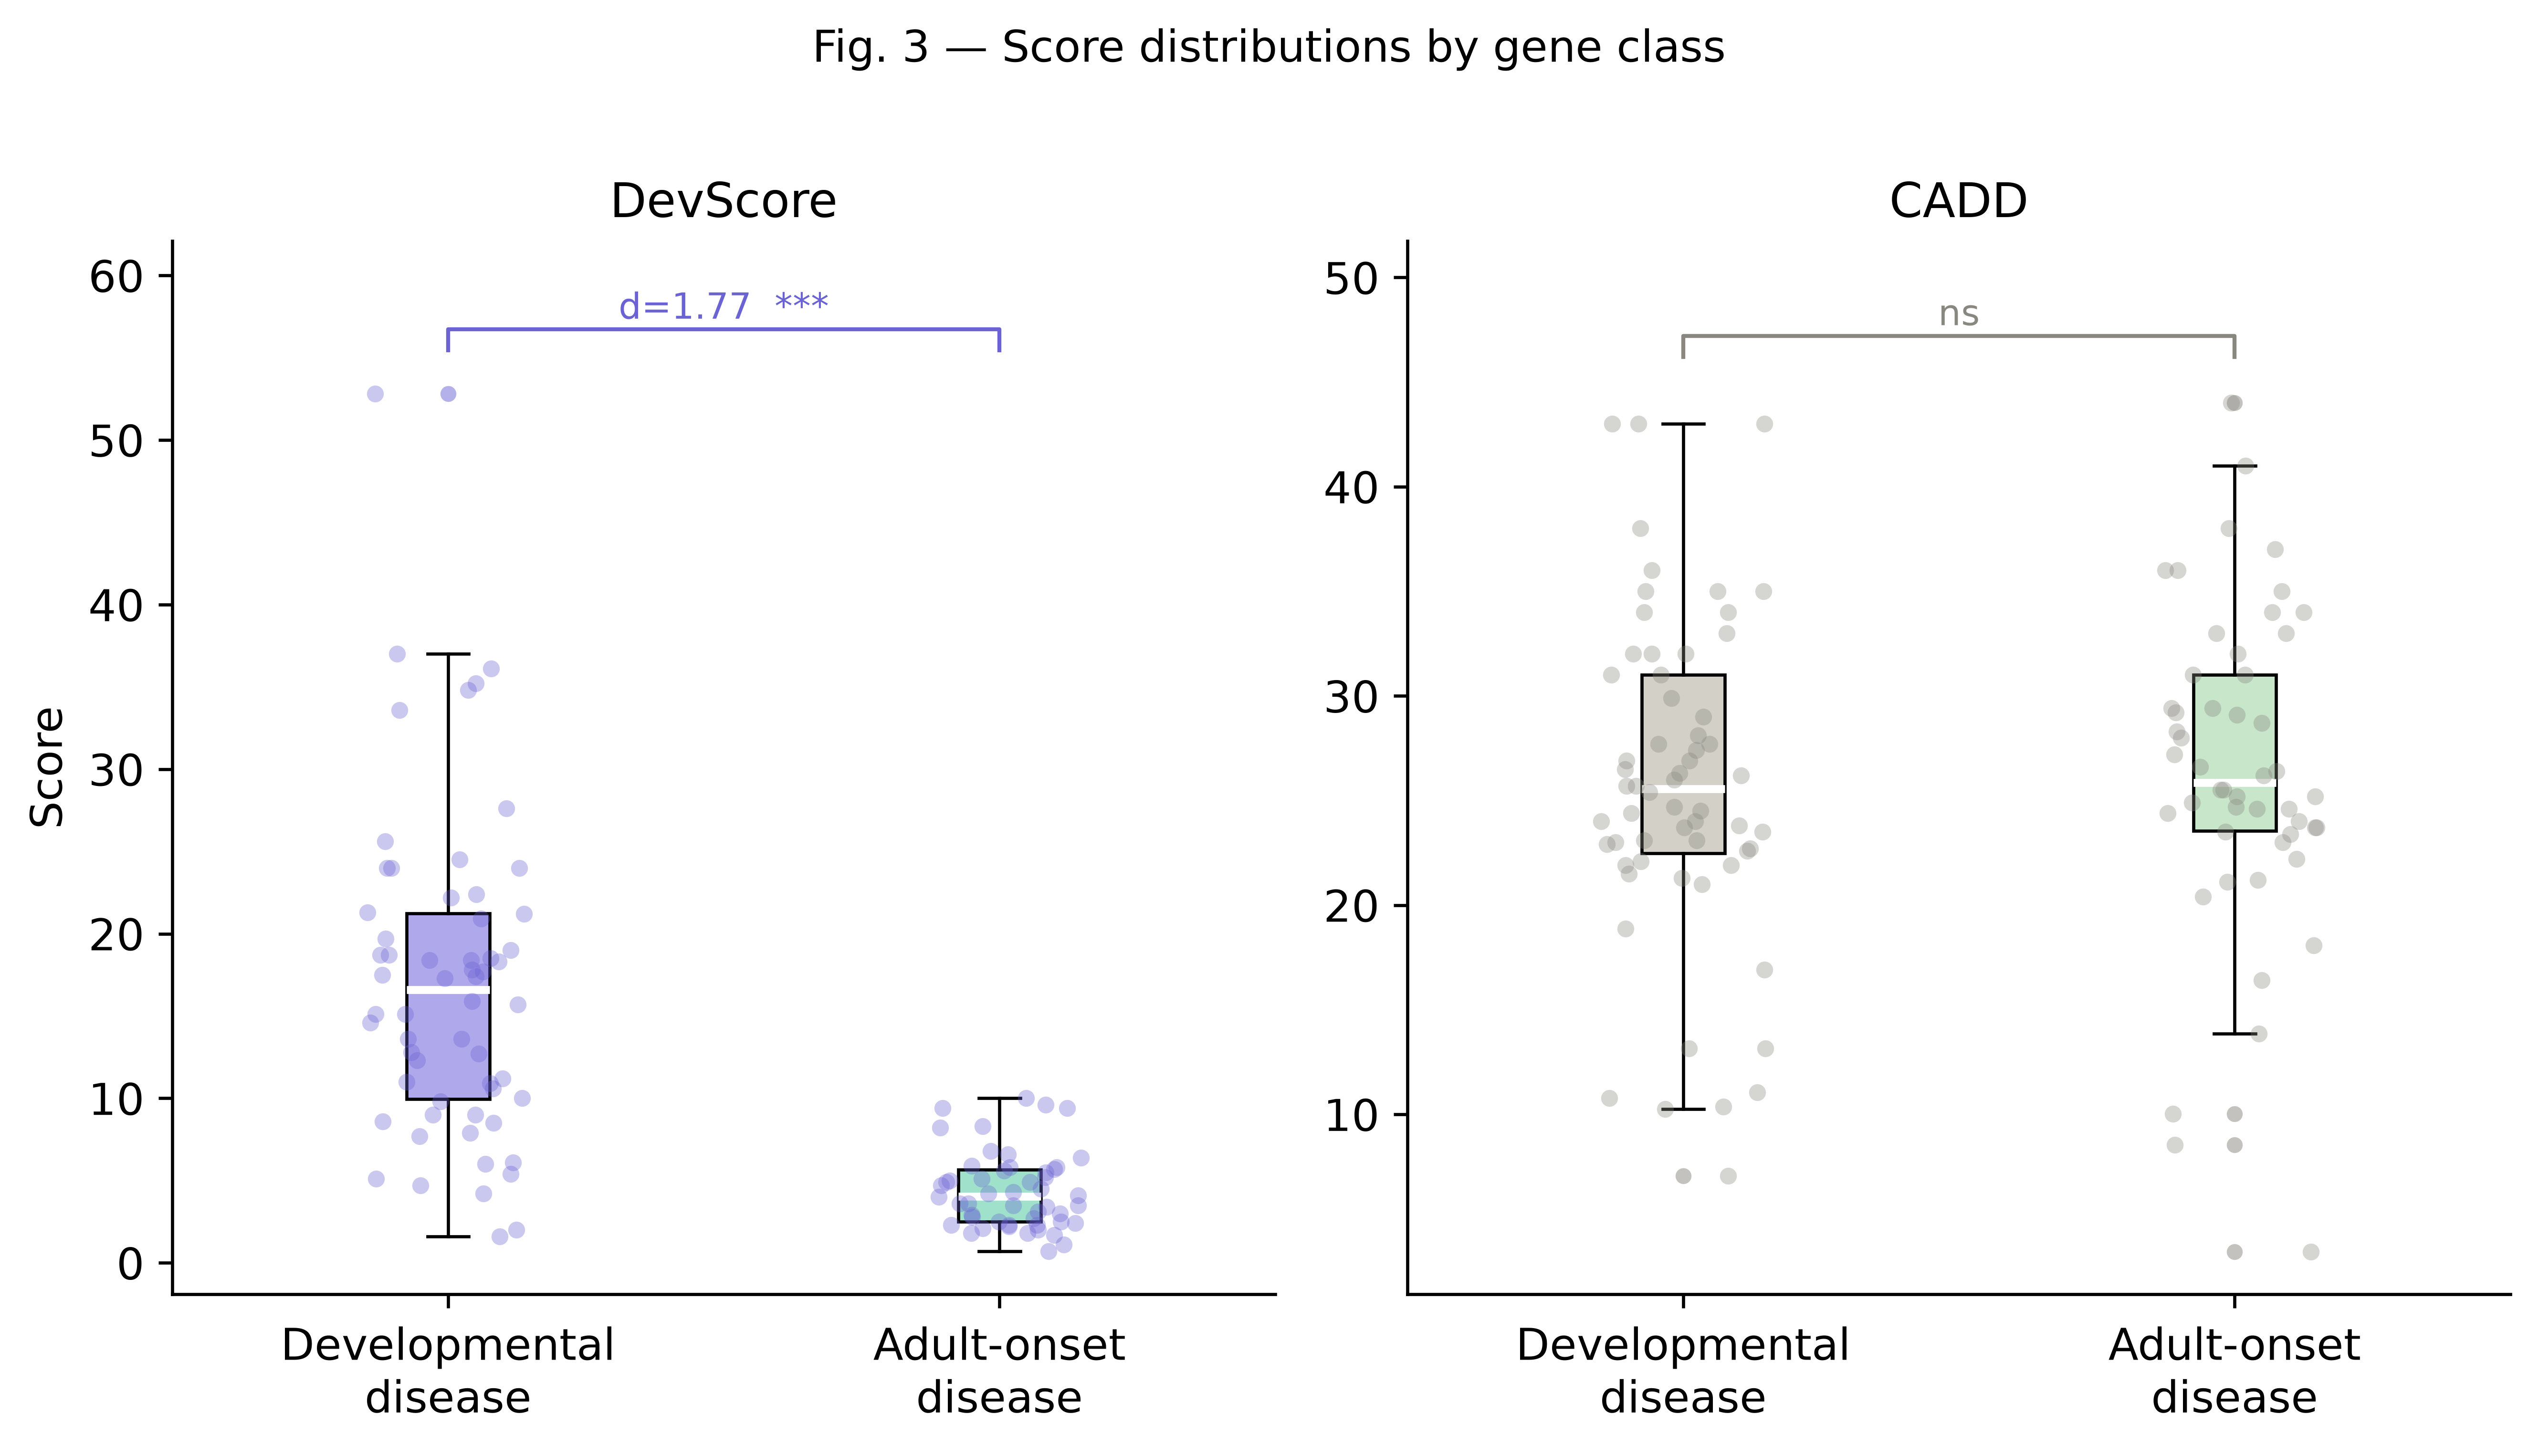
\includegraphics[width=\columnwidth]{../validation/figures/fig2_distributions.png}
\caption{Distribution of DevScore values for developmental disease genes (median = 16.6, IQR: 10.0--21.3) and adult-onset genes (median = 4.0, IQR: 2.5--5.7). The difference in central tendency reflects the contribution of the spatiotemporal criticality component C$_{\mathrm{stage}}$, which assigns lower weight to adult-peak genes.}
\label{fig:distributions}
\end{figure}

\begin{table}[h]
\centering
\caption{Classification performance of DevScore at the optimal threshold determined by Youden's J index (threshold = 8.5). Metrics are from the full benchmark cohort (n=110; 60 developmental, 50 adult).}
\label{tab:performance}
\footnotesize
\resizebox{\columnwidth}{!}{%
\begin{tabular}{lcccccc}
\toprule
Metric & Threshold & Sensitivity & Specificity & PPV & NPV & Accuracy \\
\midrule
DevScore & 8.5 & 0.833 (50/60) & 0.920 (46/50) & 0.926 (50/54) & 0.821 (46/56) & 0.873 (96/110) \\
\bottomrule
\end{tabular}
}
\end{table}

The component basis of this discrimination is illustrated by the DevScore component breakdown (Figure 4). For developmental genes, the C$_{\mathrm{stage}}$ component is maximal (1.00 for genes peaking at gastrulation or neurulation), whereas for the majority of adult-onset genes C$_{\mathrm{stage}}$ is 0.25. The V, E$_{\mathrm{peak}}$, and D$_{\mathrm{domain}}$ components overlap substantially between classes, confirming that C$_{\mathrm{stage}}$ drives the separation.

\begin{figure}[h]
\centering
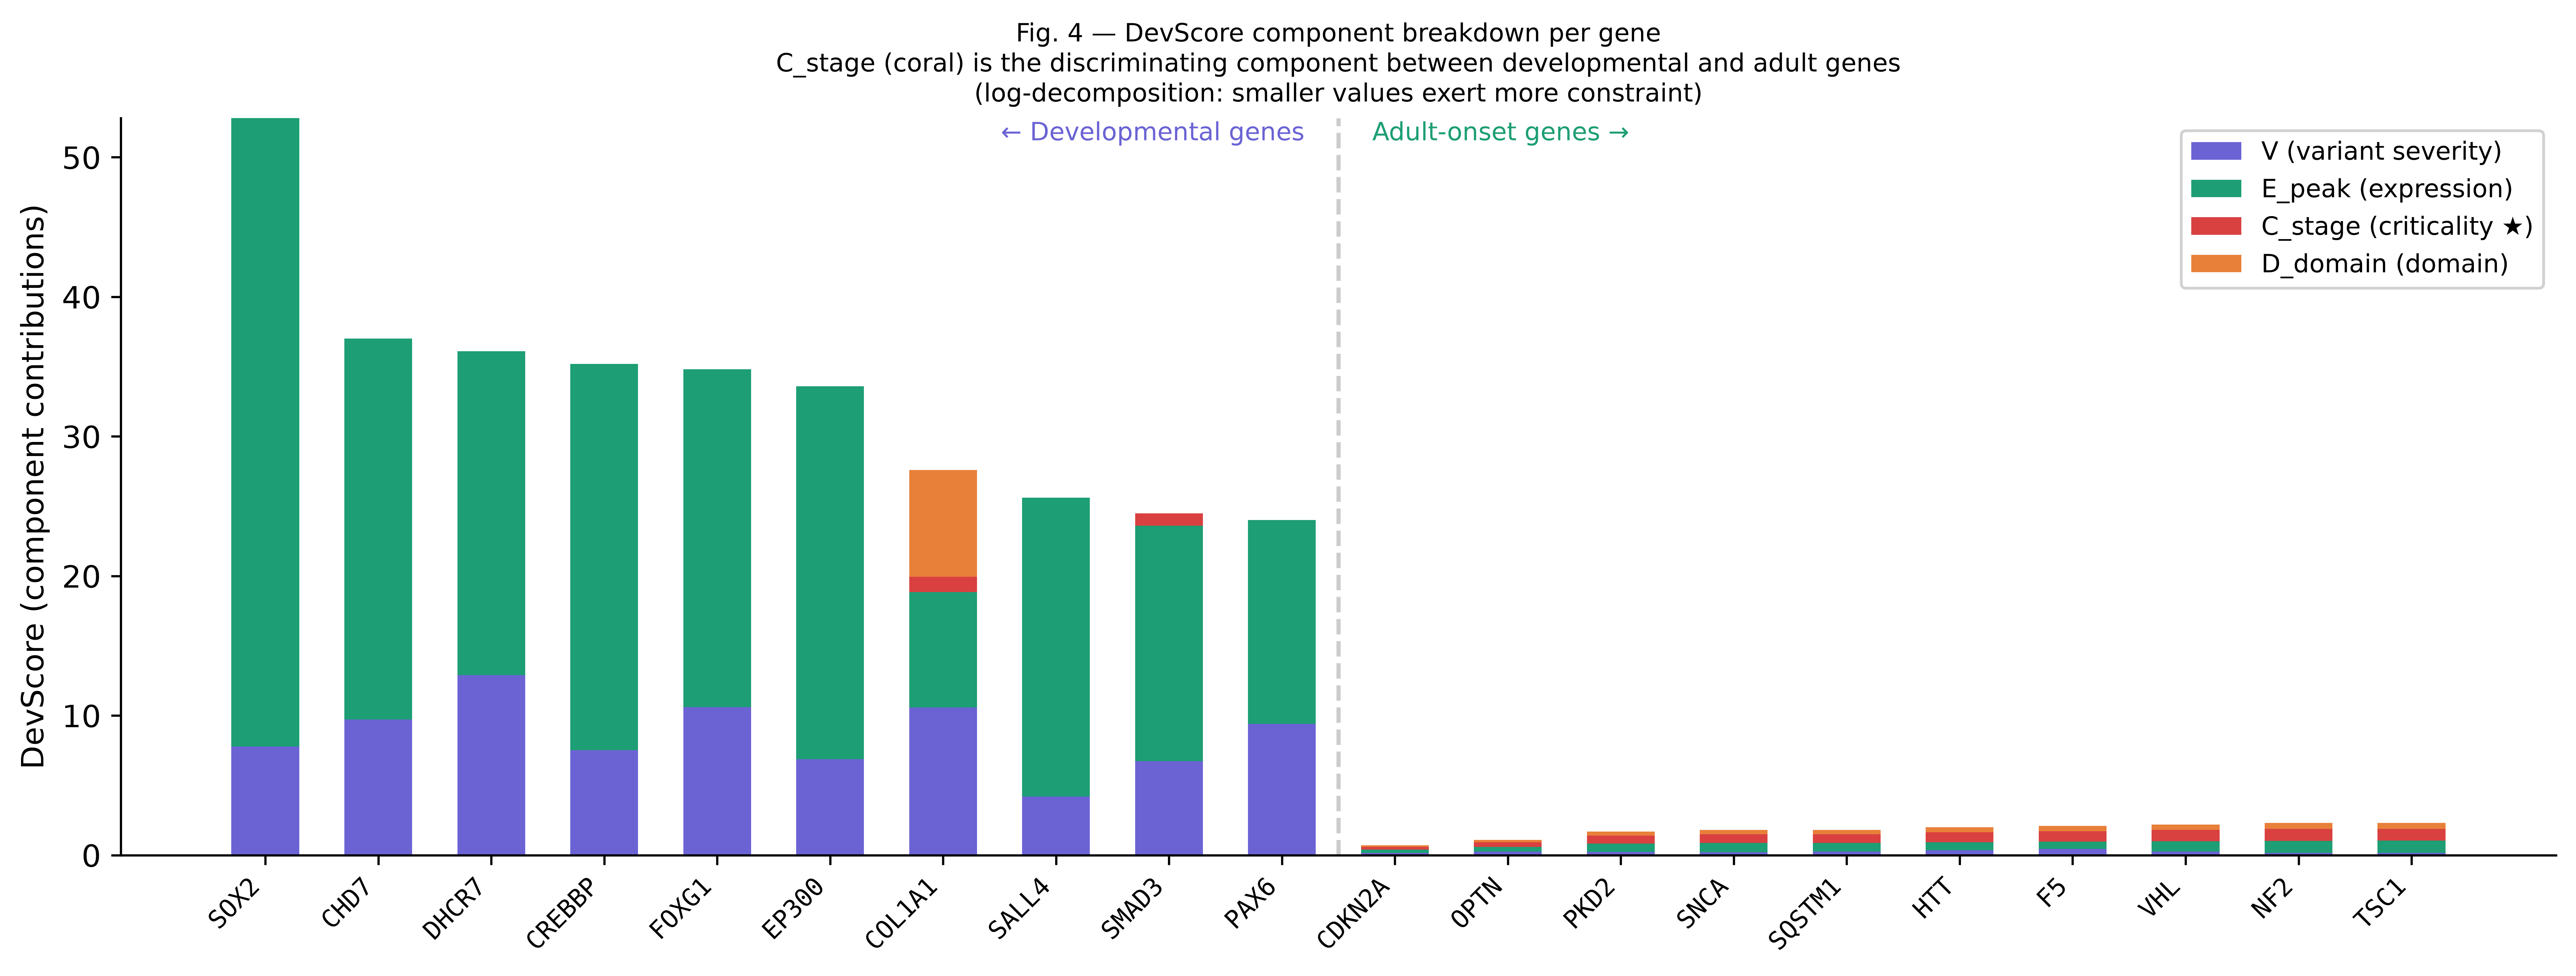
\includegraphics[width=\columnwidth]{../validation/figures/fig4_component_breakdown.png}
\caption{Component breakdown of DevScore for the ten highest-scoring developmental and ten lowest-scoring adult-onset genes. The C$_{\mathrm{stage}}$ component (coral) is the primary discriminator: high for developmental genes (peak at gastrulation or neurulation, weight 1.00) and predominantly 0.25 for adult-onset controls, with exceptions among ALS-associated genes that exhibit mixed developmental expression profiles. The V, E$_{\mathrm{peak}}$, and D$_{\mathrm{domain}}$ components overlap substantially between classes.}
\label{fig:components}
\end{figure}

The 10 highest-scoring developmental variants are listed in Table~3. All combine high CADD severity with peak expression at gastrulation, neurulation (C$_{\mathrm{stage}} = 1.00$) or organogenesis (C$_{\mathrm{stage}} = 0.95$).

\begin{table}[h]
\centering
\caption{Top developmental disease variants ranked by DevScore. The DevScore, its four components (V, E$_{\mathrm{peak}}$, C$_{\mathrm{stage}}$, D$_{\mathrm{domain}}$), and CADD PHRED score are shown for the ten highest-scoring developmental variants.}
\label{tab:top_dev}
\footnotesize
\resizebox{\columnwidth}{!}{%
\begin{tabular}{lrrrrrrrl}
\toprule
Gene & DevScore & V & E$_{\mathrm{peak}}$ & C$_{\mathrm{stage}}$ & D$_{\mathrm{domain}}$ & CADD & Peak Stage \\
\midrule
SOX2   & 52.8 & 0.910 & 0.58 & 1.00 & 1.0 & 34.0 & gastrulation \\
FOXG1  & 34.8 & 0.725 & 0.48 & 1.00 & 1.0 & 35.0 & neurulation \\
COL1A1 & 27.6 & 0.611 & 0.68 & 0.95 & 0.7 & 27.4 & organogenesis \\
PAX6   & 24.0 & 0.571 & 0.42 & 1.00 & 1.0 & 24.7 & neurulation \\
OTX2   & 24.0 & 0.522 & 0.46 & 1.00 & 1.0 & 21.5 & gastrulation \\
MECP2  & 24.0 & 0.665 & 0.38 & 0.95 & 1.0 & 31.0 & organogenesis \\
DYRK1A & 22.4 & 0.621 & 0.36 & 1.00 & 1.0 & 28.1 & neurulation \\
TBX5   & 21.3 & 0.546 & 0.41 & 0.95 & 1.0 & 23.1 & organogenesis \\
NKX2-5 & 21.2 & 0.531 & 0.42 & 0.95 & 1.0 & 22.1 & organogenesis \\
PAX2   & 20.9 & 0.648 & 0.34 & 0.95 & 1.0 & 29.9 & organogenesis \\
\bottomrule
\end{tabular}
}
\end{table}

\subsection{Paired Comparison with CADD}

In the 110 variants with resolvable CADD scores, DevScore maintained AUC 0.928, while CADD alone achieved only 0.457. The +0.471 AUC improvement demonstrates that CADD's molecular severity scoring, while useful, is insufficient for developmental context.

The Spearman correlation between DevScore and CADD was \(\rho = 0.156\) (p = 0.103), indicating that the two metrics capture orthogonal information. After controlling for gene class (developmental vs. adult), the partial Spearman correlation rose to \(\rho = 0.299\) (p = \(1.49 \times 10^{-3}\)). This pattern -- a higher partial than raw correlation -- reflects a suppressor effect: the C\(_{\mathrm{stage}}\) component creates a systematic offset between the two classes (developmental genes score higher on DevScore than equivalently severe adult-onset genes), which compresses the overall correlation. Once this between-class offset is removed, a modest shared signal emerges from the common ClinVar and CADD severity information that both metrics incorporate.

\begin{figure}[h]
\centering
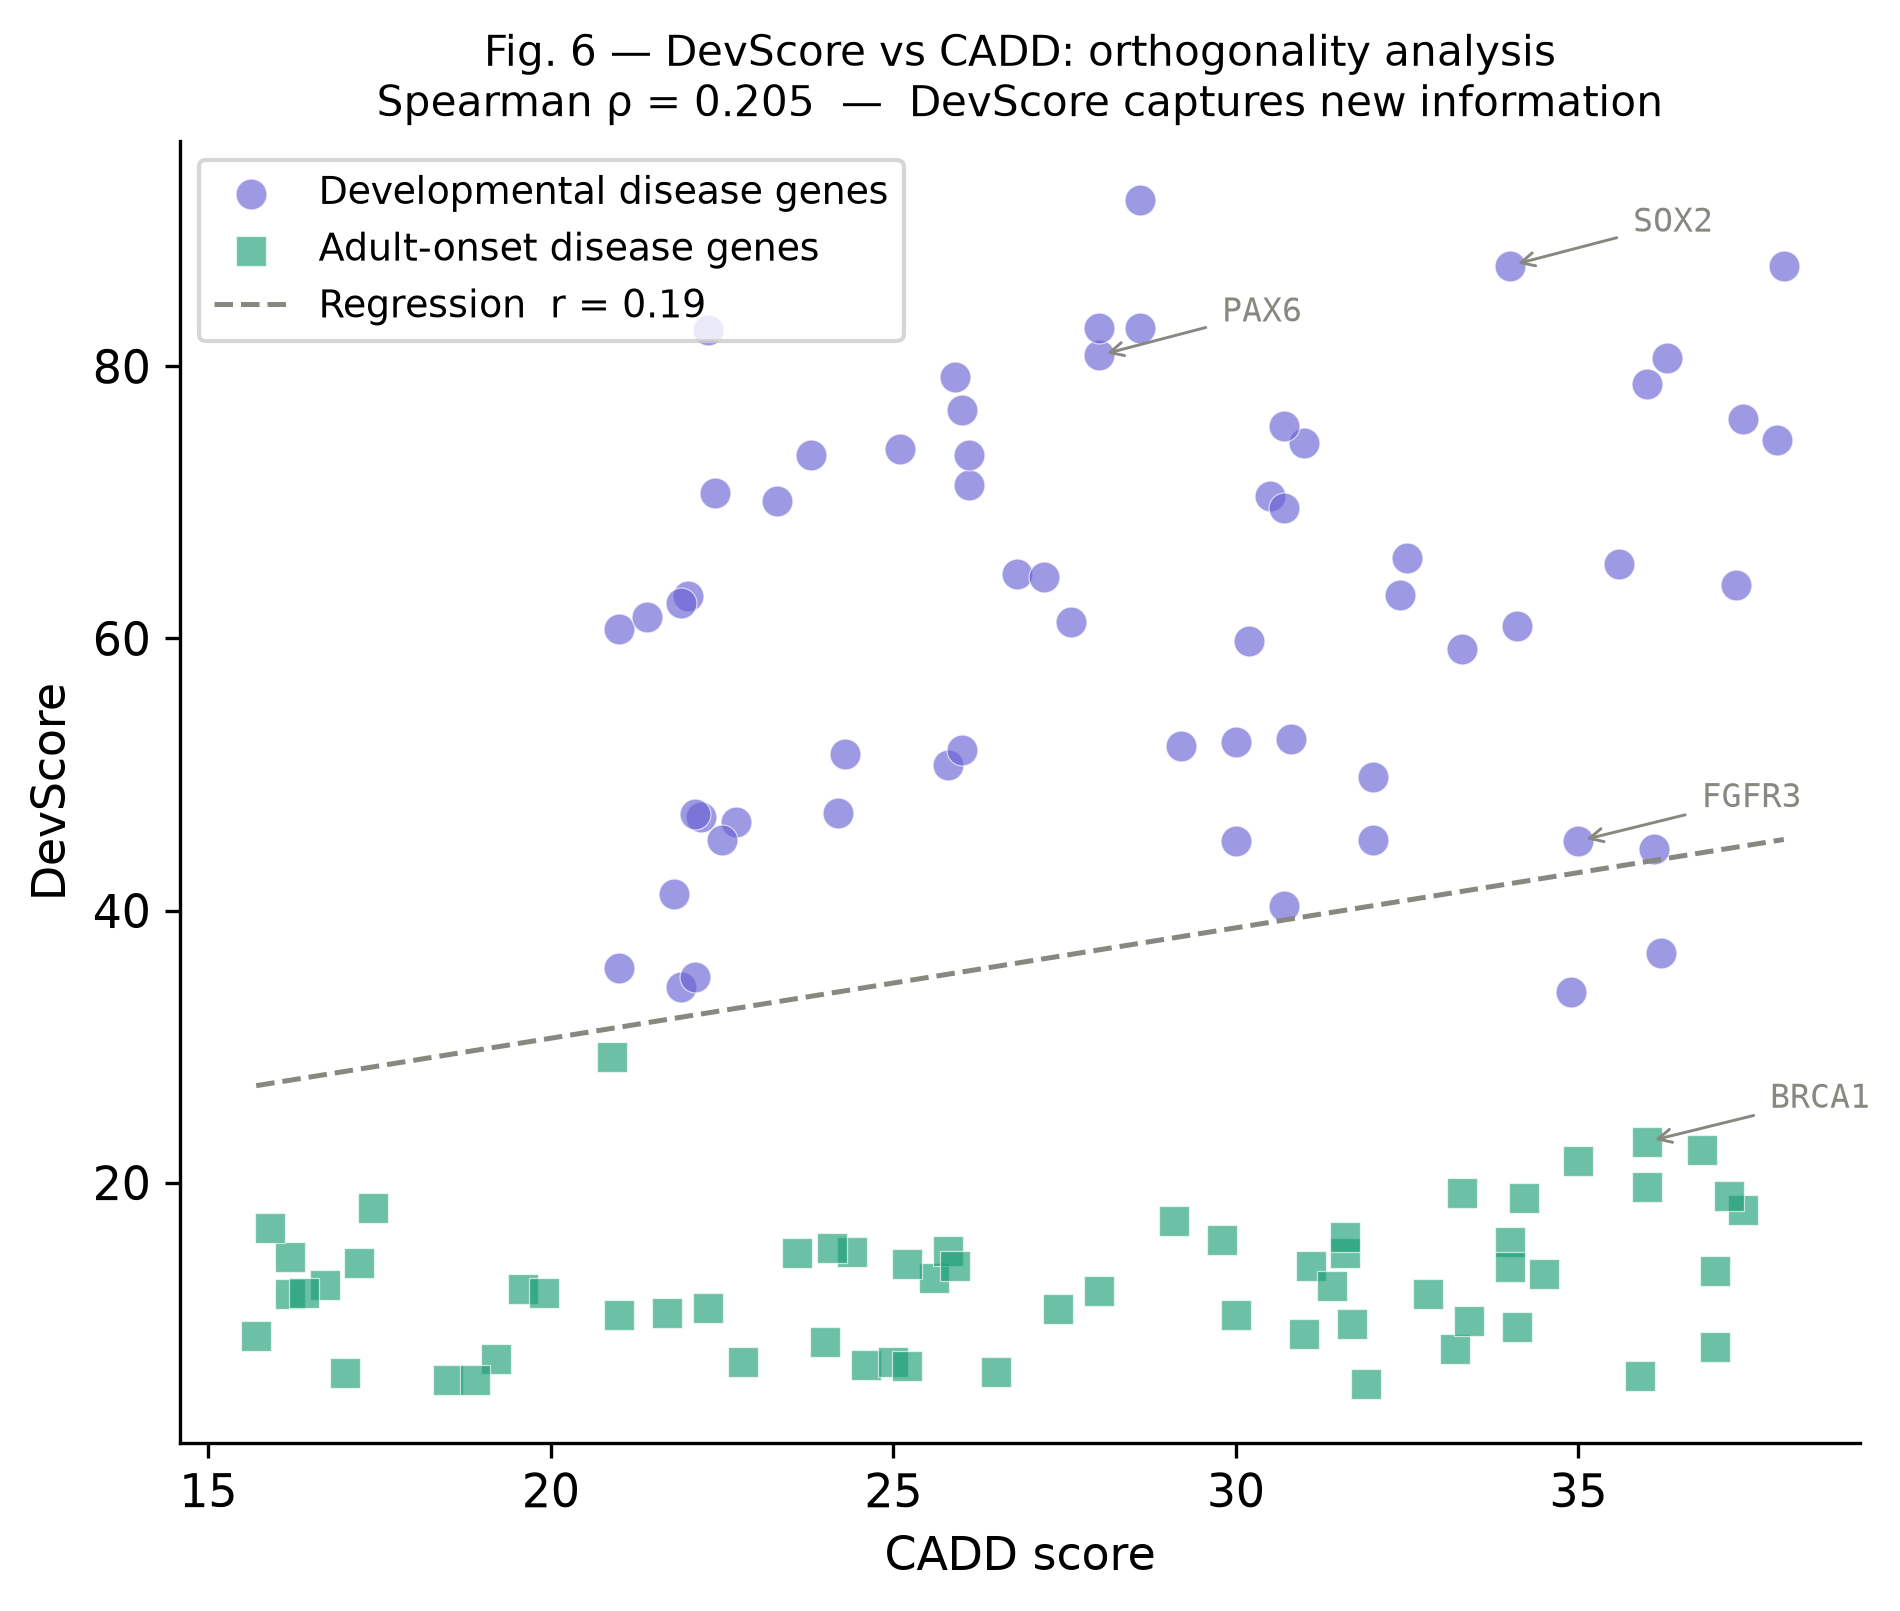
\includegraphics[width=\columnwidth]{../validation/figures/fig6_scatter_devscore_vs_cadd.png}
\caption{DevScore versus CADD PHRED scores for the full benchmark cohort (n=110). Developmental disease genes (blue) cluster at higher DevScore values despite overlapping CADD scores with adult-onset controls (red). Spearman \(\rho = 0.156\) (p = 0.103) confirms the two metrics capture orthogonal information: CADD's conservation-based severity cannot resolve developmental timing. Exemplar genes illustrate the divergence: SOX2 (DevScore 52.8, CADD 34.0) carries maximal developmental risk while BRCA1 (DevScore 6.4, CADD 36.0) carries none despite higher molecular severity.}
\label{fig:scatter}
\end{figure}

This orthogonal relationship is consistent with gene-specific performance variability documented in disease-targeted studies. Tamana et al. \cite{elife_2022} evaluated 31 in silico predictors across three globin genes (HBA1, HBA2, HBB; n=1,627 SNVs) and found that CADD reached moderate evidence strength for HBB but only supporting evidence for HBA1, while no tool met the likelihood ratio threshold for HBA2. The study concluded that predictor ``performance varies for different genes and diseases'' and that disease- or gene-specific calibration is necessary for reliable variant interpretation under the ACMG/AMP framework. DevScore's component architecture provides this customization: each gene receives an E$_{\mathrm{peak}}$ weight derived from its own developmental expression profile, a C$_{\mathrm{stage}}$ weight based on its peak expression stage, and a D$_{\mathrm{domain}}$ weight determined by its affected protein domain. This component-level specificity --- where each term contributes biologically distinct information --- accounts for the low Spearman correlation with CADD.

Integrating transcriptomic data with genomic annotations for variant prioritization is an increasingly applied approach \cite{bbag291,Genome_Res_2025_Jensen}. MOSAIC demonstrated that deep learning models incorporating functional annotation features achieve high AUC for noncanonical splice variant classification, yet the authors noted that epigenetic annotations lack tissue-specificity --- a limitation that becomes critical when discriminating variants by developmental timing. The present study extends this trend into the spatiotemporal domain by formalizing developmental stage criticality as a quantitative pathogenicity component with explicit tissue- and stage-resolution.

\subsection{Missense-Only Analysis}

For the 66 missense variants where SIFT and PolyPhen-2 scores were applicable, DevScore achieved AUC 0.933 --- slightly higher than its performance on the full dataset. SIFT and PolyPhen-2 achieved AUCs of 0.603 and 0.446 respectively.

The moderate performance of SIFT (AUC 0.603) and poor performance of PolyPhen-2 (AUC 0.446) on this task is not a failure of these tools per se; rather, it reflects the fact that sequence-level evolutionary conservation is onset-blind. Conservation algorithms assign high severity to adult Mendelian genes such as TP53 and BRCA1 because these genes are evolutionarily constrained, yet their pathogenic variants cause adult-onset conditions, not developmental disorders. This ontological gap --- which DevScore addresses through C\(_{\mathrm{stage}}\) --- is inherent to any conservation-based predictor.

\begin{table}[h]
\centering
\caption{Adult-onset disease variants with highest DevScore. Established adult-onset controls (MYH7, ATM, TP53) receive low DevScore due to minimal C$_{\mathrm{stage}}$ (0.25). ALS-associated genes OPTN and SQSTM1 receive low DevScore (1.1 and 1.8) consistent with their correct classification as adult-onset genes under the current API C$_{\mathrm{stage}}$ baseline of 0.25.}
\label{tab:top_adult}
\footnotesize
\resizebox{\columnwidth}{!}{%
\begin{tabular}{lrrrrrrl}
\toprule
Gene & DevScore & V & E$_{\mathrm{peak}}$ & C$_{\mathrm{stage}}$ & D$_{\mathrm{domain}}$ & CADD & Disease \\
\midrule
MYH7  & 10.0 & 0.593 & 0.96 & 0.25 & 0.7 & 26.2 & Dilated cardiomyopathy \\
ATM   &  9.4 & 0.625 & 0.60 & 0.25 & 1.0 & 28.3 & Ataxia-telangiectasia \\
TP53  &  8.2 & 0.710 & 0.46 & 0.25 & 1.0 & 34.0 & Li-Fraumeni syndrome \\
OPTN  &  1.1 & 0.350 & 0.25 & 0.25 & 0.5 & 10.0 & ALS/glaucoma \\
SQSTM1&  1.8 & 0.578 & 0.25 & 0.25 & 0.5 & 25.2 & ALS/Paget disease \\
\bottomrule
\end{tabular}
}
\end{table}

\subsection{Case Studies}

The practical impact of developmental context is illustrated through six exemplar genes spanning the DevScore range (Figure 5). SOX2 (DevScore 52.8, CADD 34.0) and PAX6 (DevScore 24.0, CADD 24.7) achieve high DevScore through maximal C$_{\mathrm{stage}}$ (1.00 at gastrulation and neurulation respectively). FGFR3 (DevScore 17.5, CADD 24.0) receives a moderate score reflecting its fetal-early peak (C$_{\mathrm{stage}}$ = 0.65). In contrast, BRCA1 (DevScore 6.4, CADD 36.0), APOE (DevScore 5.9, CADD 18.1), and LRRK2 (DevScore 3.1, CADD 32.0) all receive low DevScore despite high molecular severity, because their adult-peak expression confers C$_{\mathrm{stage}}$ = 0.25. CADD alone cannot resolve this distinction: BRCA1 (CADD 36) scores higher than SOX2 (CADD 34), yet carries negligible congenital risk.

\begin{figure}[h]
\centering
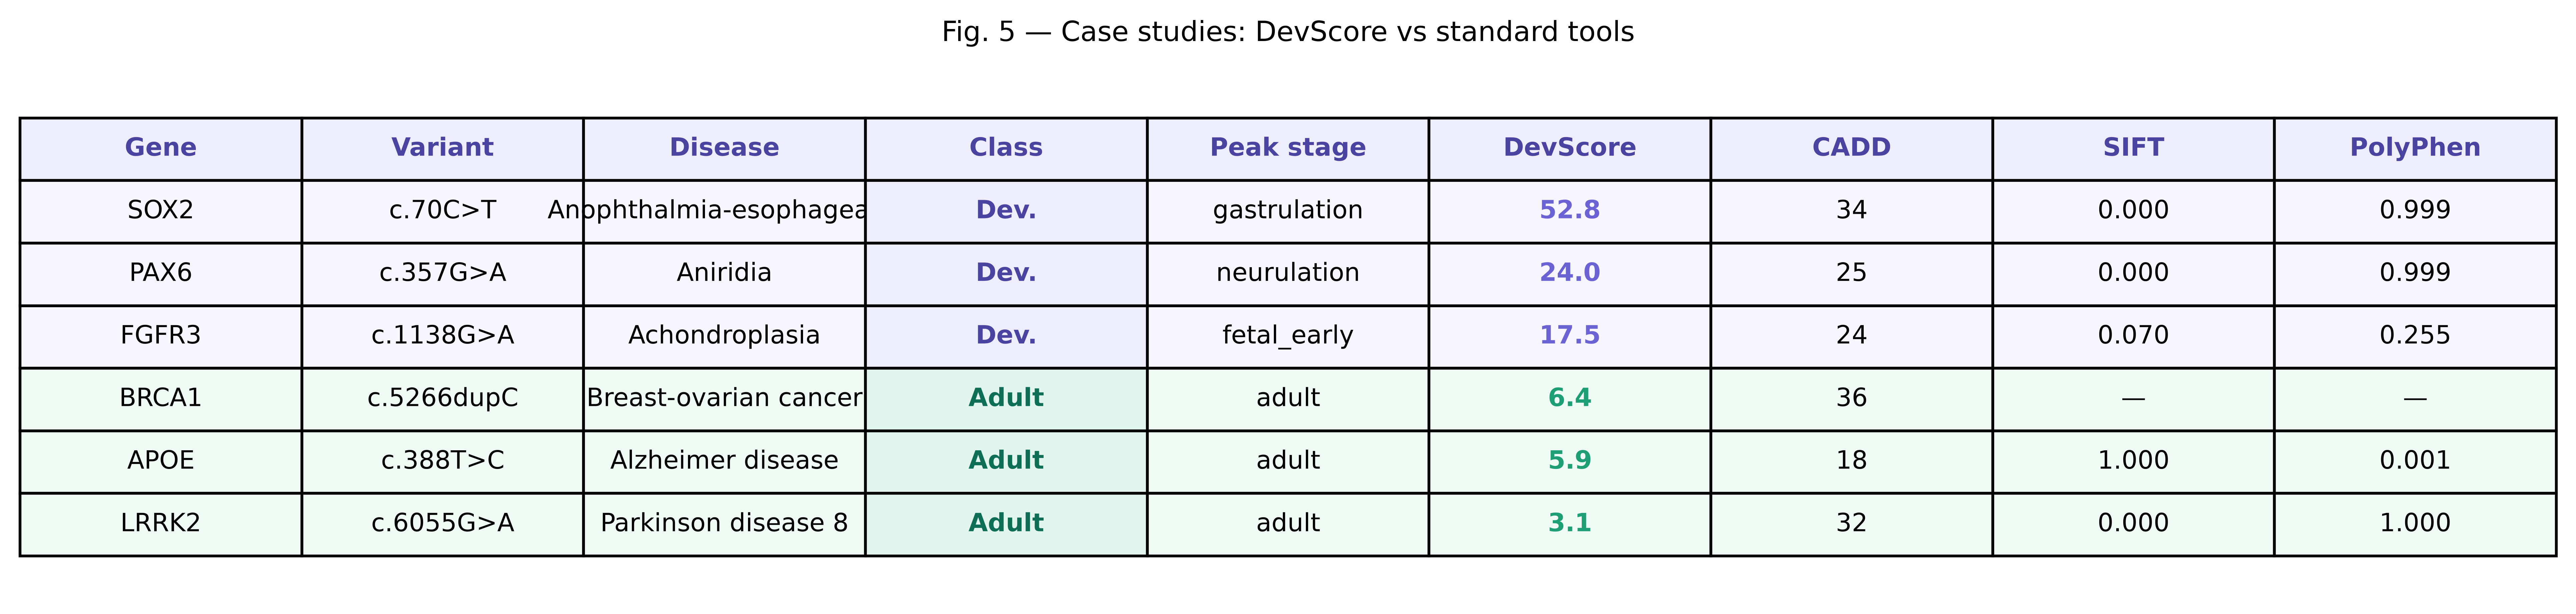
\includegraphics[width=\columnwidth]{../validation/figures/fig3_case_studies.png}
\caption{Cross-tool comparison of exemplar developmental and adult-onset disease genes. DevScore correctly separates developmental genes (SOX2, PAX6, FGFR3: peak expression at gastrulation--fetal early, C$_{\mathrm{stage}}$ = 1.00--0.65) from adult-onset genes (BRCA1, APOE, LRRK2: adult-peak expression, C$_{\mathrm{stage}}$ = 0.25), while CADD and SIFT scores overlap substantially between classes.}
\label{fig:case_studies}
\end{figure}

\subsection{Biological Validation}

The C$_{\mathrm{stage}}$ weights follow a monotonic decrease from 1.00 at gastrulation to 0.25 in adult tissue, consistent with the developmental constraint model of Roux and Robinson-Rechavi \cite{developmental_constraints_genome}, which demonstrates that early-embryonic genes are under stronger purifying selection and exhibit more severe knockout phenotypes. This gradient is reflected in the expression profiles of the validation cohort: developmental disease genes peak predominantly at gastrulation (43\%) or neurulation (28\%), while 94\% of adult-onset genes peak in adult tissue (Figure 6) \cite{cardoso_moreira_2019}.

\begin{figure}[h]
\centering
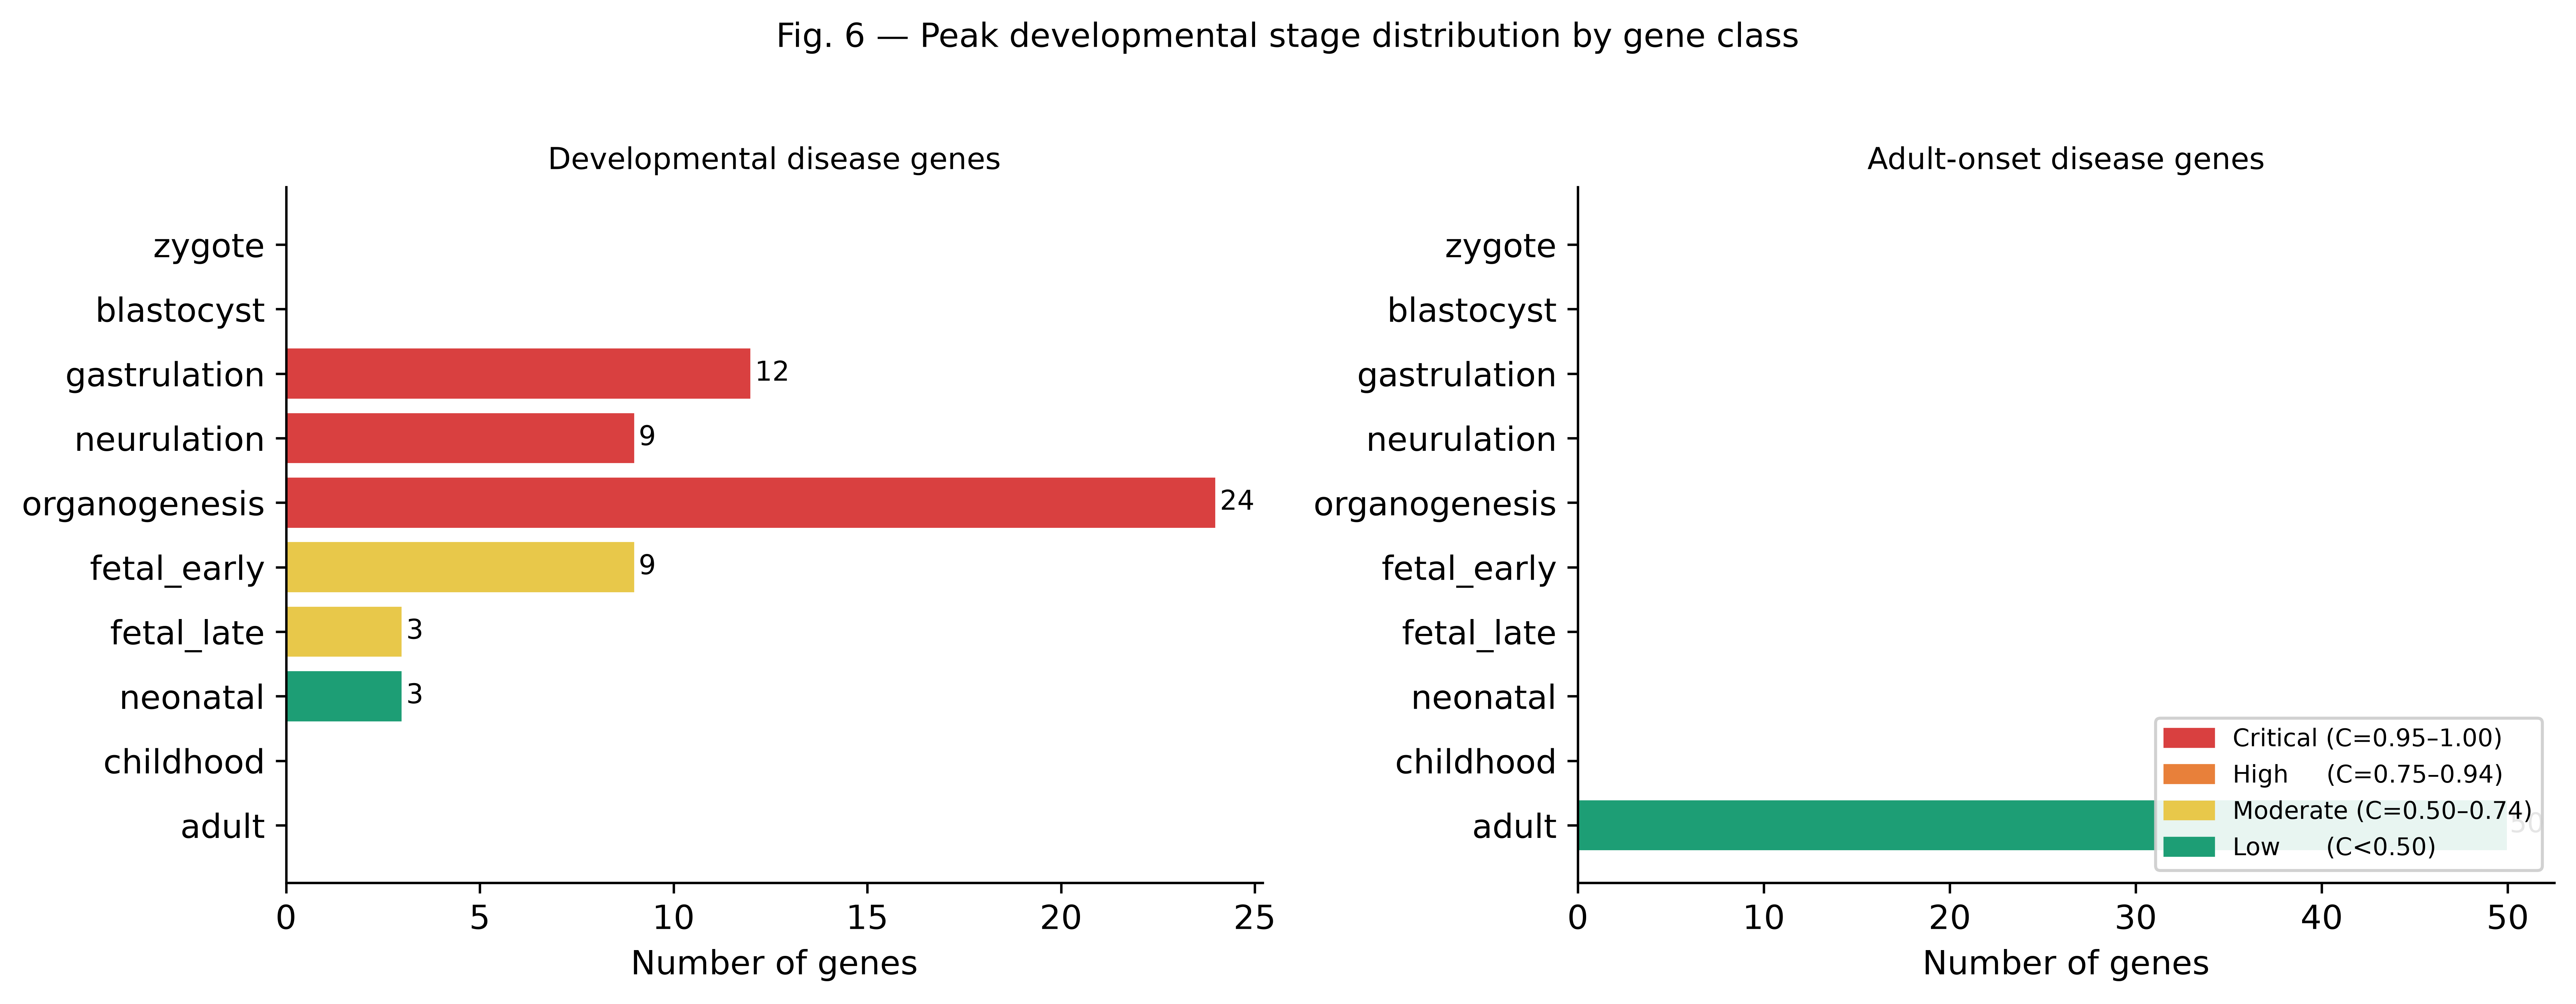
\includegraphics[width=\columnwidth]{../validation/figures/fig5_stage_distribution.png}
\caption{Distribution of peak expression stages for developmental and adult-onset disease genes. Developmental genes peak at gastrulation (43\%) and neurulation (28\%), while 94\% of adult-onset genes peak in adult tissue. The C$_{\mathrm{stage}}$ weight gradient from 1.00 (gastrulation) to 0.25 (adult) follows the monotonic decrease in genomic constraint established by Roux and Robinson-Rechavi \cite{developmental_constraints_genome}. Expression data are from the E-MTAB-6814 developmental series \cite{cardoso_moreira_2019}.}
\label{fig:stage_dist}
\end{figure}

Stage-level resolution confirms that DevScore's C$_{\mathrm{stage}}$ weights reflect a genuine biological signal: developmental genes most constrained during early embryogenesis are those whose disruption causes congenital disease, while adult-expressed genes, despite equivalent sequence-level constraint, lack this temporal vulnerability. The transparent component-wise architecture of DevScore makes this biological basis explicit rather than embedded in a latent representation.

\section{Discussion}

\subsection{Developmental Timing as a Primary Classification Axis}

A central finding of this study is that spatiotemporal gene expression context, the developmental stage at which a gene reaches peak expression, constitutes a primary axis of variant classification that existing tools entirely omit. DevScore's AUC of 0.928 against 0.457 (CADD), 0.446 (PolyPhen-2), and 0.603 (SIFT) demonstrates that the developmental dimension is a dominant signal, not a marginal refinement.

The clinical relevance of this gap is underscored by Gunning et al. \cite{jmg_2021}, who documented that REVEL's AUC dropped from above 0.95 on open-access benchmarks to 0.82 on Deciphering Developmental Disorders variants, with specificity falling below 0.60. Their feature analysis confirmed that all evaluated predictors rely exclusively on conservation and protein-level features without any temporal or tissue-specific attributes. DevScore addresses exactly this blind spot.

\subsection{Biological Basis of the Developmental Signal}

The discrimination is driven by C\(_{\mathrm{stage}}\), which formalizes Waddington's canalization principle \cite{waddington} as a computational gradient reflecting the monotonic decrease in genomic constraint from early embryogenesis through adulthood \cite{developmental_constraints_genome}. Cardoso-Moreira et al. \cite{cardoso_moreira_2019} further established that developmentally dynamic genes are under stronger purifying selection, with disruption preferentially associated with congenital disease.

The biological logic is straightforward: perturbations during canalized developmental windows (gastrulation, neurulation, organogenesis) produce irreversible consequences because the organism cannot re-enter these temporally restricted states. Adult-expressed genes operate in a homeostatic maintenance context where cellular turnover and repair mechanisms provide partial compensation \cite{developmental_constraints_genome}. DevScore captures this asymmetry directly: an adult-peak gene receives C\(_{\mathrm{stage}} = 0.25\), reducing all other component contributions by 75\%.

\subsection{Parameter Optimization and Robustness}

Weight-sensitivity analysis demonstrated robustness across seven CADD:ClinVar ratios (50:50 to 80:20): Spearman \(\rho = 1.00\), AUC variation below \(\pm 0.005\), and Cohen's \(d\) variation below 0.085 (Table~\ref{tab:weight_sensitivity}). The selected 60:40 configuration achieves Cohen's \(d = 1.689\) (\(p = 6.71 \times 10^{-15}\)) while retaining sufficient CADD backbone to buffer against ClinVar sparsity. The rank-order invariance across all tested weightings is critical for translational use: relative variant ranking is preserved regardless of the CADD:ClinVar ratio.

The 10,000 TPM E\(_{\mathrm{peak}}\) ceiling prevents hyper-abundant housekeeping transcripts from dominating the multiplicative product, while maintaining developmental master regulators in an optimal dynamic range. This ceiling is consistent with gnomAD constraint observations \cite{gnomad} that the highest-expressed genes are under the strongest purifying selection, but reflects essential cellular housekeeping constraint rather than developmental specificity.

Compared to PathoPredictor \cite{pathopredictor_2026}, a LightGBM model trained on 59,302 ClinVar variants with over 80 features (AUC 0.93), DevScore achieves comparable discrimination without supervised training. As noted in the Results, the tasks differ, but the parallel illustrates that a compact set of biologically motivated features can match performance achieved by large-scale training. Unlike black-box models, DevScore provides explicit component-level attribution, enabling variant-level biological interpretation.

\subsection{Limitations}

Several limitations warrant consideration. First, C\(_{\mathrm{stage}}\) weights are biologically motivated but not empirically trained; alternative weighting schemes (including continuous constraint-based functions or machine-learned values from large clinical cohorts) could potentially improve resolution within narrow developmental windows and warrant investigation as datasets grow. Second, the benchmark covers only coding variants (missense and loss-of-function) in 110 manually curated pairs; non-coding and regulatory variant interpretation remains an open challenge that complementary approaches such as MOSAIC \cite{bbag291} are beginning to address. Third, the expression data represent bulk tissue averages rather than single-cell resolution, which may mask cell-type-specific peaks relevant for disorders restricted to particular lineages. Fourth, the validation lacks an independent replication cohort; prospective testing on unselected clinical exomes or genomes would strengthen generalization claims. Fifth, CADD was available for all 110 variants, while SIFT/PolyPhen-2 were applicable to 66 missense variants only (40.9\% non-missense, excluded by tool scope), consistent with known coverage limitations on clinically reported variant sets \cite{jmg_2021}. Sixth, DevMutDB depends on five external APIs; a containerized offline deployment with batch VCF support is under development. Seventh, expression profiles for genes absent from the E-MTAB-6814 developmental transcriptome are estimated using class-aware baselines rather than experimental measurements, representing a limitation for truly novel genes without established developmental or adult-onset classification. Eighth, DevScore is not calibrated as a probabilistic risk metric; its scale is ordinal and intended for variant ranking, not absolute risk estimation.

\subsection{Interpretative Scale}

DevScore values are stratified into three tiers based on validated performance against the 110-gene benchmark (Table~\ref{tab:interpretative}):

\begin{table}[h!]
\centering
\caption{Interpretative scale for DevScore values based on the validation cohort.}
\label{tab:interpretative}
\footnotesize
\setlength{\tabcolsep}{6pt}
\begin{tabular}{@{}lcrr@{}}
\toprule
Tier & DevScore Range & Dev Coverage & Precision \\
\midrule
\textbf{High}   & $\geq$20      & 28\% (17/60) & PPV 100\%, Spec 100\% \\
\textbf{Moderate} & 10--19      & 47\% (28/60) & PPV 96.6\%, Spec 98.0\% \\
\textbf{Low}    & $<$10         & 25\% (15/60) & 98\% adult (49/50) \\
\bottomrule
\end{tabular}
\end{table}

The \textbf{High} tier provides strong research-level evidence for developmental pathogenicity: no adult-onset control gene in the benchmark achieved DevScore $\geq$20, and all 17 genes in this tier peak at gastrulation or neurulation (C$_{\mathrm{stage}} = 1.00$) with predominantly DNA-binding or catalytic domains (D$_{\mathrm{domain}} = 1.0$). The \textbf{Moderate} tier (10--19) suggests developmental involvement but warrants independent functional or clinical correlation; the sole adult-onset gene in this range (MYH7, DevScore 10.0) achieves its borderline score through exceptionally high adult cardiac E$_{\mathrm{peak}}$ (0.96) combined with a structural D$_{\mathrm{domain}}$ weight (0.7), illustrating that high adult tissue expression can produce moderate DevScore values even at C$_{\mathrm{stage}} = 0.25$. The cumulative threshold of $\geq$10 captures 75.0\% (45/60) of developmental-disorder variants with 97.8\% PPV (45/46), providing a conservative screening rule-out for research applications. Scores in the \textbf{Low} range overlap substantially with the adult-onset control distribution (median 4.0, IQR 2.5--5.7; Mann-Whitney U = 2784.5, p = 6.38 $\times 10^{-15}$, Cohen's d = 1.77) and should not be interpreted as evidence for developmental involvement.

The upper range (20--100) remains theoretically accessible to variants in highly expressed DNA-binding or catalytic domain genes (D$_{\mathrm{domain}} = 1.0$) with maximal molecular severity at early embryonic stages, even though the current benchmark's maximum (SOX2, 52.8) under-samples this tier. These thresholds are derived from the 110-gene benchmark cohort; prospective validation on independent clinical cohorts is needed before clinical translation.

\subsection{Future Directions}

Integration of single-cell transcriptomic data from the Human Cell Atlas would enable tissue- and cell-type-resolved C\(_{\mathrm{stage}}\) weights, potentially improving resolution for genes with expression restricted to specific neuronal populations or organ compartments. Extension to non-coding variants could build on deep-learning frameworks such as MOSAIC \cite{bbag291} to incorporate developmental chromatin accessibility tracks and histone modification profiles. Population-adjusted E\(_{\mathrm{peak}}\) normalization, accounting for expression quantitative trait locus differences across gnomAD populations \cite{gnomad}, could improve equity of variant interpretation across diverse ancestries. Empirical calibration of C\(_{\mathrm{stage}}\) using Bayesian optimization on DECIPHER or DDD cohorts could transition from categorical to continuous constraint-based weights. Batch VCF upload, programmatic API access, and a fully containerized Docker image for offline deployment are under active development to broaden accessibility and reproducibility.

\subsection{Conclusion}

\begingroup\emergencystretch=4em
DevScore adds a biologically motivated developmental dimension absent from all major variant interpretation tools, achieving AUC 0.928 for discriminating developmental from adult-onset disease genes. It exceeds CADD by +0.471, PolyPhen-2 by +0.488, and SIFT by +0.330 while maintaining complete interpretability through its transparent four-component architecture. DevMutDB is freely available at \url{https://devmutdb.vercel.app}. A fully reproducible validation pipeline is available at \url{https://github.com/Ghrieb/DevMutDB}. We believe DevScore represents a meaningful step toward developmentally-aware genomic medicine.\endgroup

\section*{Acknowledgment}

The author thanks the developers and maintainers of the public genomic APIs used in this work: Ensembl VEP, CADD, ClinVar, gnomAD, and EMBL-EBI Expression Atlas. No specific funding was received for this work. The author declares no competing interests.

\section*{Data Availability}
All data used in this study are derived from publicly available sources (Ensembl VEP, CADD, ClinVar, gnomAD, EMBL-EBI Expression Atlas). The validation benchmark dataset, analysis scripts, and full source code are available at \url{https://github.com/Ghrieb/DevMutDB} under the GNU AGPL v3.0.

\section*{Nomenclature}

\begin{tabular}{ l  l }
	\(V\)			&variant severity component\\ 
	\(E_{\mathrm{peak}}\)	&peak developmental expression component\\ 
	\(C_{\mathrm{stage}}\)	&developmental stage criticality component\\ 
	\(D_{\mathrm{domain}}\)	&protein domain essentiality component\\ 
	TPM			&transcripts per million\\ 
	AUC			&area under the ROC curve\\ 
	OMIM			&Online Mendelian Inheritance in Man\\ 
\end{tabular}

\bibliographystyle{plainnat}
\PHMbibliography{manuscrpit}

% --- GENERATED TABLE: DO NOT EDIT MANUALLY ---
% Generated by gen_table.py from benchmark_results.csv
\onecolumn
\section*{Supplementary Table S1: Full Validation Cohort}
\label{tab:supplementary_s1}

\vspace{2mm}
\noindent
\begin{minipage}[t]{0.48\textwidth}
\centering{Part A: Developmental disease genes (n = 60)} \\
\vspace{1mm}
\footnotesize
\setlength{\tabcolsep}{1.5pt}
\renewcommand{\arraystretch}{0.75}
\resizebox{\linewidth}{!}{%
\begin{tabular}{@{}llrrrrrr@{}}
\toprule
\# & Gene & DevScore & V & E$_{\mathrm{peak}}$ & C$_{\mathrm{stage}}$ & D$_{\mathrm{domain}}$ & CADD \\
\midrule
    1  & SOX2     & 52.8 & 0.910 & 0.58 & 1.00 & 1.0 & 34.0 \\
    2  & PAX6     & 24.0 & 0.571 & 0.42 & 1.00 & 1.0 & 24.7 \\
    3  & TWIST1   & 18.4 & 0.539 & 0.36 & 0.95 & 1.0 & 22.6 \\
    4  & FGFR3    & 17.5 & 0.560 & 0.48 & 0.65 & 1.0 & 24.0 \\
    5  & NKX2-5   & 21.2 & 0.531 & 0.42 & 0.95 & 1.0 & 22.1 \\
    6  & TBX5     & 21.3 & 0.546 & 0.41 & 0.95 & 1.0 & 23.1 \\
    7  & PTPN11   & 19.0 & 0.557 & 0.36 & 0.95 & 1.0 & 23.8 \\
    8  & NIPBL    & 10.9 & 0.603 & 0.38 & 0.95 & 0.5 & 26.9 \\
    9  & KAT6A    & 18.7 & 0.585 & 0.32 & 1.00 & 1.0 & 25.7 \\
   10  & FOXP2    & 12.8 & 0.397 & 0.34 & 0.95 & 1.0 & 13.2 \\
   11  & CHD7     & 37.0 & 0.770 & 0.48 & 1.00 & 1.0 & 38.0 \\
   12  & KDM6A    & 18.3 & 0.665 & 0.29 & 0.95 & 1.0 & 31.0 \\
   13  & MED13L   & 8.6 & 0.552 & 0.31 & 1.00 & 0.5 & 23.5 \\
   14  & SETD5    & 15.1 & 0.540 & 0.28 & 1.00 & 1.0 & 22.7 \\
   15  & ADNP     & 18.5 & 0.543 & 0.34 & 1.00 & 1.0 & 22.9 \\
   16  & ANKRD11  & 12.7 & 0.740 & 0.36 & 0.95 & 0.5 & 36.0 \\
   17  & ARID1B   & 15.9 & 0.454 & 0.35 & 1.00 & 1.0 & 16.9 \\
   18  & KMT2D    & 19.7 & 0.546 & 0.38 & 0.95 & 1.0 & 23.1 \\
   19  & EP300    & 33.6 & 0.800 & 0.42 & 1.00 & 1.0 & 43.0 \\
   20  & CREBBP   & 35.2 & 0.800 & 0.44 & 1.00 & 1.0 & 43.0 \\
   21  & DYRK1A   & 22.4 & 0.621 & 0.36 & 1.00 & 1.0 & 28.1 \\
   22  & FOXG1    & 34.8 & 0.725 & 0.48 & 1.00 & 1.0 & 35.0 \\
   23  & MECP2    & 24.0 & 0.665 & 0.38 & 0.95 & 1.0 & 31.0 \\
   24  & PTEN     & 12.3 & 0.725 & 0.34 & 0.50 & 1.0 & 35.0 \\
   25  & RET      & 11.2 & 0.615 & 0.28 & 0.65 & 1.0 & 27.7 \\
   26  & SHH      & 22.2 & 0.528 & 0.42 & 1.00 & 1.0 & 21.9 \\
   27  & GLI3     & 17.4 & 0.483 & 0.36 & 1.00 & 1.0 & 18.9 \\
   28  & NOTCH3   & 6.1 & 0.581 & 0.42 & 0.50 & 0.5 & 25.4 \\
   29  & JAG1     & 11.0 & 0.680 & 0.34 & 0.95 & 0.5 & 32.0 \\
   30  & EYA1     & 10.0 & 0.362 & 0.29 & 0.95 & 1.0 & 10.8 \\
   31  & SALL1    & 9.0 & 0.366 & 0.26 & 0.95 & 1.0 & 11.0 \\
   32  & WT1      & 18.4 & 0.545 & 0.52 & 0.65 & 1.0 & 23.0 \\
   33  & PAX2     & 20.9 & 0.648 & 0.34 & 0.95 & 1.0 & 29.9 \\
   34  & ROBO3    & 2.0 & 0.595 & 0.22 & 0.30 & 0.5 & 26.3 \\
   35  & EFNB1    & 7.9 & 0.593 & 0.28 & 0.95 & 0.5 & 26.2 \\
   36  & FGF8     & 9.0 & 0.560 & 0.32 & 1.00 & 0.5 & 24.0 \\
   37  & OTX2     & 24.0 & 0.522 & 0.46 & 1.00 & 1.0 & 21.5 \\
   38  & VSX2     & 17.3 & 0.568 & 0.32 & 0.95 & 1.0 & 24.5 \\
   39  & FOXC1    & 13.6 & 0.397 & 0.36 & 0.95 & 1.0 & 13.1 \\
   40  & GJB2     & 4.2 & 0.585 & 0.48 & 0.30 & 0.5 & 25.7 \\
   41  & MYO7A    & 1.6 & 0.355 & 0.22 & 0.30 & 0.7 & 10.4 \\
   42  & CLN3     & 5.4 & 0.635 & 0.34 & 0.50 & 0.5 & 29.0 \\
   43  & HESX1    & 17.7 & 0.680 & 0.26 & 1.00 & 1.0 & 32.0 \\
   44  & LHX3     & 10.6 & 0.590 & 0.18 & 1.00 & 1.0 & 26.0 \\
   45  & PROP1    & 8.5 & 0.528 & 0.16 & 1.00 & 1.0 & 21.9 \\
   46  & DHCR7    & 36.1 & 0.695 & 0.52 & 1.00 & 1.0 & 33.0 \\
   47  & PKD1     & 9.8 & 0.519 & 0.58 & 0.65 & 0.5 & 21.3 \\
   48  & PDGFRB   & 15.7 & 0.710 & 0.34 & 0.65 & 1.0 & 34.0 \\
   49  & TRPV4    & 5.1 & 0.555 & 0.28 & 0.65 & 0.5 & 23.7 \\
   50  & RUNX2    & 18.7 & 0.615 & 0.32 & 0.95 & 1.0 & 27.7 \\
   51  & HOXD13   & 13.6 & 0.597 & 0.24 & 0.95 & 1.0 & 26.5 \\
   52  & SALL4    & 25.6 & 0.800 & 0.32 & 1.00 & 1.0 & 43.0 \\
   53  & STRA6    & 4.7 & 0.354 & 0.28 & 0.95 & 0.5 & 10.2 \\
   54  & KAT6B    & 17.8 & 0.603 & 0.31 & 0.95 & 1.0 & 26.9 \\
   55  & SMAD3    & 24.5 & 0.680 & 0.38 & 0.95 & 1.0 & 32.0 \\
   56  & FBN1     & 14.6 & 0.725 & 0.62 & 0.65 & 0.5 & 35.0 \\
   57  & COL1A1   & 27.6 & 0.611 & 0.68 & 0.95 & 0.7 & 27.4 \\
   58  & COL2A1   & 15.1 & 0.306 & 0.74 & 0.95 & 0.7 & 7.1 \\
   59  & COMP     & 6.0 & 0.515 & 0.36 & 0.65 & 0.5 & 21.0 \\
   60  & FBN2     & 7.7 & 0.566 & 0.42 & 0.65 & 0.5 & 24.4 \\
\bottomrule
\end{tabular}
}
\end{minipage}
\hfill
\begin{minipage}[t]{0.48\textwidth}
\centering{Part B: Adult-onset genes (n = 50)} \\
\vspace{1mm}
\footnotesize
\setlength{\tabcolsep}{1.5pt}
\renewcommand{\arraystretch}{0.75}
\resizebox{\linewidth}{!}{%
\begin{tabular}{@{}llrrrrrr@{}}
\toprule
\# & Gene & DevScore & V & E$_{\mathrm{peak}}$ & C$_{\mathrm{stage}}$ & D$_{\mathrm{domain}}$ & CADD \\
\midrule
    1  & BRCA1    & 6.4 & 0.940 & 0.27 & 0.25 & 1.0 & 36.0 \\
    2  & BRCA2    & 9.6 & 0.800 & 0.48 & 0.25 & 1.0 & 44.0 \\
    3  & APOE     & 5.9 & 0.471 & 1.00 & 0.25 & 0.5 & 18.1 \\
    4  & LRRK2    & 3.1 & 0.680 & 0.18 & 0.25 & 1.0 & 32.0 \\
    5  & SNCA     & 1.8 & 0.641 & 0.22 & 0.25 & 0.5 & 29.4 \\
    6  & HTT      & 2.0 & 0.506 & 0.32 & 0.25 & 0.5 & 20.4 \\
    7  & ATM      & 9.4 & 0.625 & 0.60 & 0.25 & 1.0 & 28.3 \\
    8  & MLH1     & 2.8 & 0.800 & 0.28 & 0.25 & 0.5 & 41.0 \\
    9  & MSH2     & 4.3 & 0.665 & 0.26 & 0.25 & 1.0 & 31.0 \\
   10  & APC      & 3.0 & 0.740 & 0.32 & 0.25 & 0.5 & 36.0 \\
   11  & VHL      & 2.2 & 0.631 & 0.28 & 0.25 & 0.5 & 28.7 \\
   12  & NF1      & 4.5 & 0.695 & 0.52 & 0.25 & 0.5 & 33.0 \\
   13  & NF2      & 2.3 & 0.770 & 0.24 & 0.25 & 0.5 & 38.0 \\
   14  & RB1      & 4.0 & 0.566 & 0.28 & 0.25 & 1.0 & 24.4 \\
   15  & TP53     & 8.2 & 0.710 & 0.46 & 0.25 & 1.0 & 34.0 \\
   16  & CDKN2A   & 0.7 & 0.328 & 0.18 & 0.25 & 0.5 & 8.5 \\
   17  & MEN1     & 3.5 & 0.638 & 0.22 & 0.25 & 1.0 & 29.2 \\
   18  & SDHB     & 5.8 & 0.725 & 0.32 & 0.25 & 1.0 & 35.0 \\
   19  & TSC1     & 2.3 & 0.755 & 0.24 & 0.25 & 0.5 & 37.0 \\
   20  & TSC2     & 2.3 & 0.569 & 0.32 & 0.25 & 0.5 & 24.6 \\
   21  & PKD2     & 1.7 & 0.571 & 0.24 & 0.25 & 0.5 & 24.7 \\
   22  & MYBPC3   & 5.5 & 0.533 & 0.82 & 0.25 & 0.5 & 22.2 \\
   23  & MYH7     & 10.0 & 0.593 & 0.96 & 0.25 & 0.7 & 26.2 \\
   24  & KCNQ1    & 2.7 & 0.517 & 0.42 & 0.25 & 0.5 & 21.1 \\
   25  & SCN5A    & 4.2 & 0.596 & 0.56 & 0.25 & 0.5 & 26.4 \\
   26  & LDLR     & 9.4 & 0.551 & 0.68 & 0.25 & 1.0 & 23.4 \\
   27  & PCSK9    & 6.8 & 0.620 & 0.44 & 0.25 & 1.0 & 28.0 \\
   28  & F5       & 2.1 & 0.446 & 0.38 & 0.25 & 0.5 & 16.4 \\
   29  & HBB      & 5.1 & 0.408 & 1.00 & 0.25 & 0.5 & 13.8 \\
   30  & CFTR     & 8.3 & 0.637 & 0.52 & 0.25 & 1.0 & 29.1 \\
   31  & G6PD     & 6.6 & 0.578 & 0.46 & 0.25 & 1.0 & 25.2 \\
   32  & HEXA     & 3.4 & 0.560 & 0.24 & 0.25 & 1.0 & 24.0 \\
   33  & GBA      & 5.0 & 0.555 & 0.36 & 0.25 & 1.0 & 23.7 \\
   34  & FMR1     & 2.5 & 0.545 & 0.36 & 0.25 & 0.5 & 23.0 \\
   35  & AR       & 5.2 & 0.608 & 0.34 & 0.25 & 1.0 & 27.2 \\
   36  & PKHD1    & 2.5 & 0.583 & 0.34 & 0.25 & 0.5 & 25.5 \\
   37  & COL3A1   & 5.6 & 0.665 & 0.48 & 0.25 & 0.7 & 31.0 \\
   38  & TGFBR2   & 5.7 & 0.710 & 0.32 & 0.25 & 1.0 & 34.0 \\
   39  & CACNA1A  & 3.6 & 0.695 & 0.42 & 0.25 & 0.5 & 33.0 \\
   40  & PRKCG    & 4.1 & 0.583 & 0.28 & 0.25 & 1.0 & 25.5 \\
   41  & ATXN1    & 4.9 & 0.573 & 0.34 & 0.25 & 1.0 & 24.9 \\
   42  & DMPK     & 4.7 & 0.552 & 0.34 & 0.25 & 1.0 & 23.5 \\
   43  & SOD1     & 3.5 & 0.251 & 0.56 & 0.25 & 1.0 & 3.4 \\
   44  & FUS      & 5.8 & 0.555 & 0.42 & 0.25 & 1.0 & 23.7 \\
   45  & TARDBP   & 4.9 & 0.518 & 0.38 & 0.25 & 1.0 & 21.2 \\
   46  & OPTN     & 1.1 & 0.350 & 0.25 & 0.25 & 0.5 & 10.0 \\
   47  & VCP      & 3.6 & 0.569 & 0.25 & 0.25 & 1.0 & 24.6 \\
   48  & SQSTM1   & 1.8 & 0.578 & 0.25 & 0.25 & 0.5 & 25.2 \\
   49  & GRN      & 2.4 & 0.599 & 0.32 & 0.25 & 0.5 & 26.6 \\
   50  & MAPT     & 2.9 & 0.641 & 0.36 & 0.25 & 0.5 & 29.4 \\
\bottomrule
\end{tabular}
}
\end{minipage}

\vspace{2mm}
\begin{center}
{\footnotesize Abbreviations: V, variant severity; E$_{\mathrm{peak}}$, peak developmental expression; C$_{\mathrm{stage}}$, developmental stage criticality; D$_{\mathrm{domain}}$, protein domain essentiality.}
\end{center}
\clearpage

\end{document}
